% Section content template for individual Educative lessons
% This file contains the actual content for a specific section
% Generated from Educative API section content

% Section: Getting Ready: The ATM System
% Section ID: 5101998182760448
% Section Slug: getting-ready-the-atm-system
% Generated: 2025-12-12T15:53:03.338167

\subsection{Problem definition}\label{GdBbXiDwBbAsUwxqCLfX8}
\\
An \textbf{automated teller machine (ATM)} is a self-service terminal that enables bank customers to perform financial transactions without interacting with a human teller or visiting a physical bank branch. Through ATMs, users can perform essential banking operations such as depositing cash, withdrawing money, checking account balances, and transferring funds between accounts. ATMs are typically placed in accessible public locations like banks, malls, airports, and convenience stores to provide round-the-clock banking services.
\\
In this LLD interview case study, you'll focus on:

\begin{itemize}
\item
\protect\phantomsection\label{htpsYQvYvLGsPYm1hu5Ys}
Enabling secure card-based access and PIN verification for users.
\item
\protect\phantomsection\label{kO-BfabYNDyfRrsGzeV1p}
Supporting core transactions: cash withdrawal, deposit, balance inquiry, and fund transfer.
\item
\protect\phantomsection\label{LuhirYsFAalXIGaMVxWCZ}
Managing cash inventory within the ATM, including withdrawal limits and handling insufficient funds.
\item
\protect\phantomsection\label{Irs0VCOoDsae4rKxtA5qZ}
Ensuring a seamless and secure user experience through well-coordinated hardware and software components.
\end{itemize}
\\
\textbf{Note:} The design can be adapted for modern ATMs with features like contactless cards, mobile integrations, or advanced security (e.g., biometrics), but we will focus on the core ATM functionalities.

\begin{figure}[htbp]
 \centering
 \begin{subfigure}[b]{0.48\textwidth}
 \centering
 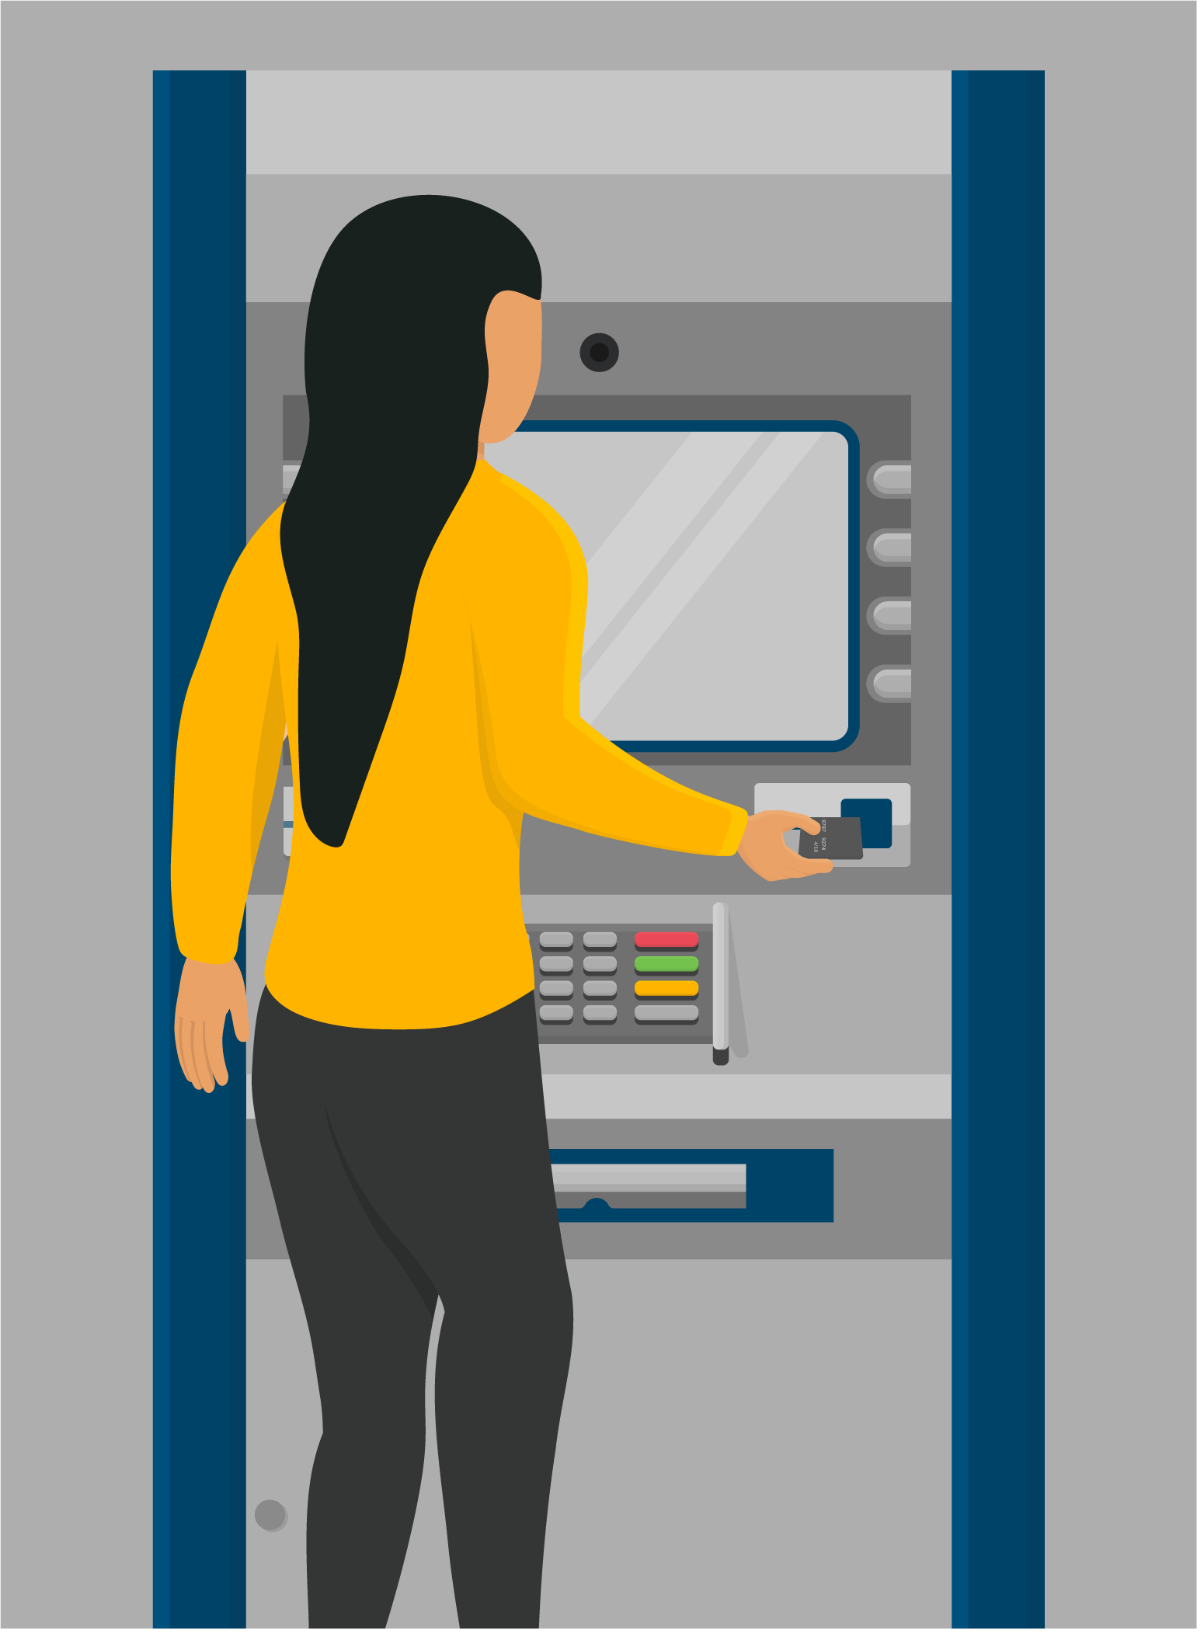
\includegraphics[width=\textwidth]{Images/chapter_16/section_5101998182760448/6088952475025408.png}
 \caption{The user inserts their card in the ATM}
 \end{subfigure}
 \hfill
 \begin{subfigure}[b]{0.48\textwidth}
 \centering
 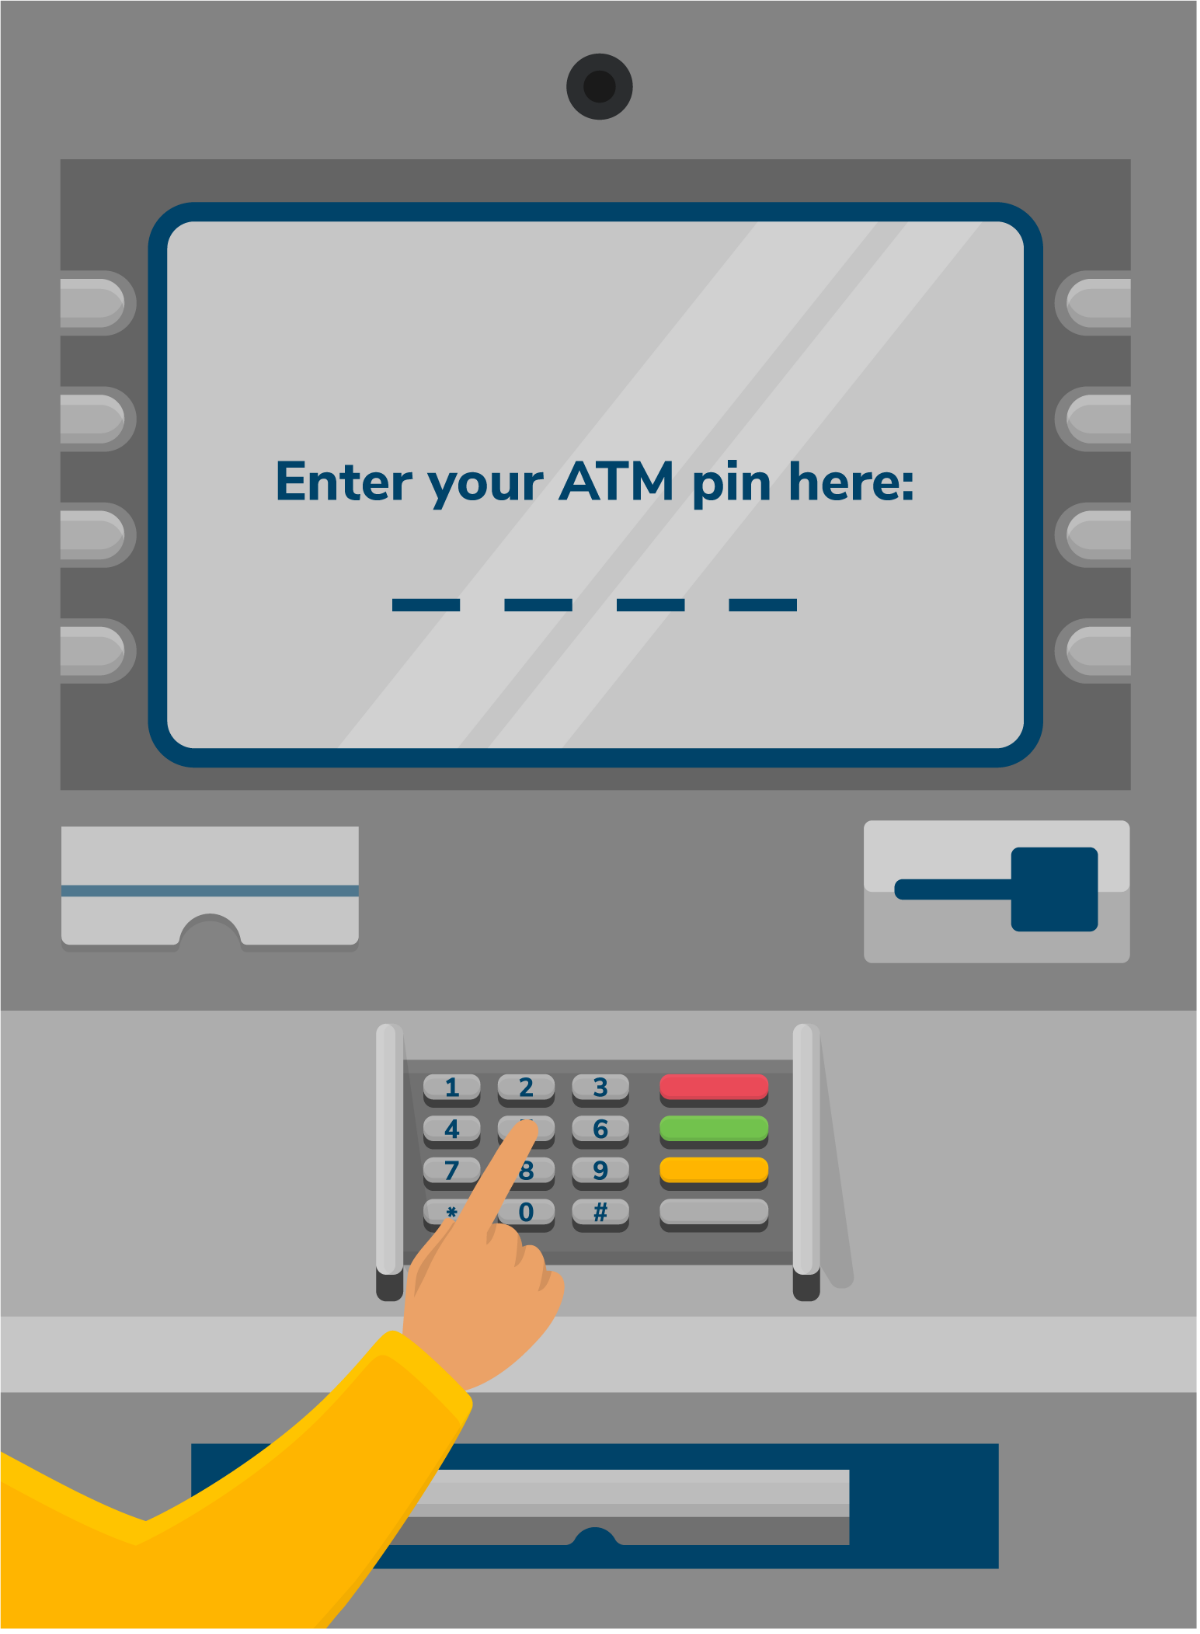
\includegraphics[width=\textwidth]{Images/chapter_16/section_5101998182760448/5125340239495168.png}
 \caption{The ATM reads the information on the card and prompts the user to enter their PIN}
 \end{subfigure}
\end{figure}

\begin{figure}[htbp]
 \centering
 \begin{subfigure}[b]{0.48\textwidth}
 \centering
 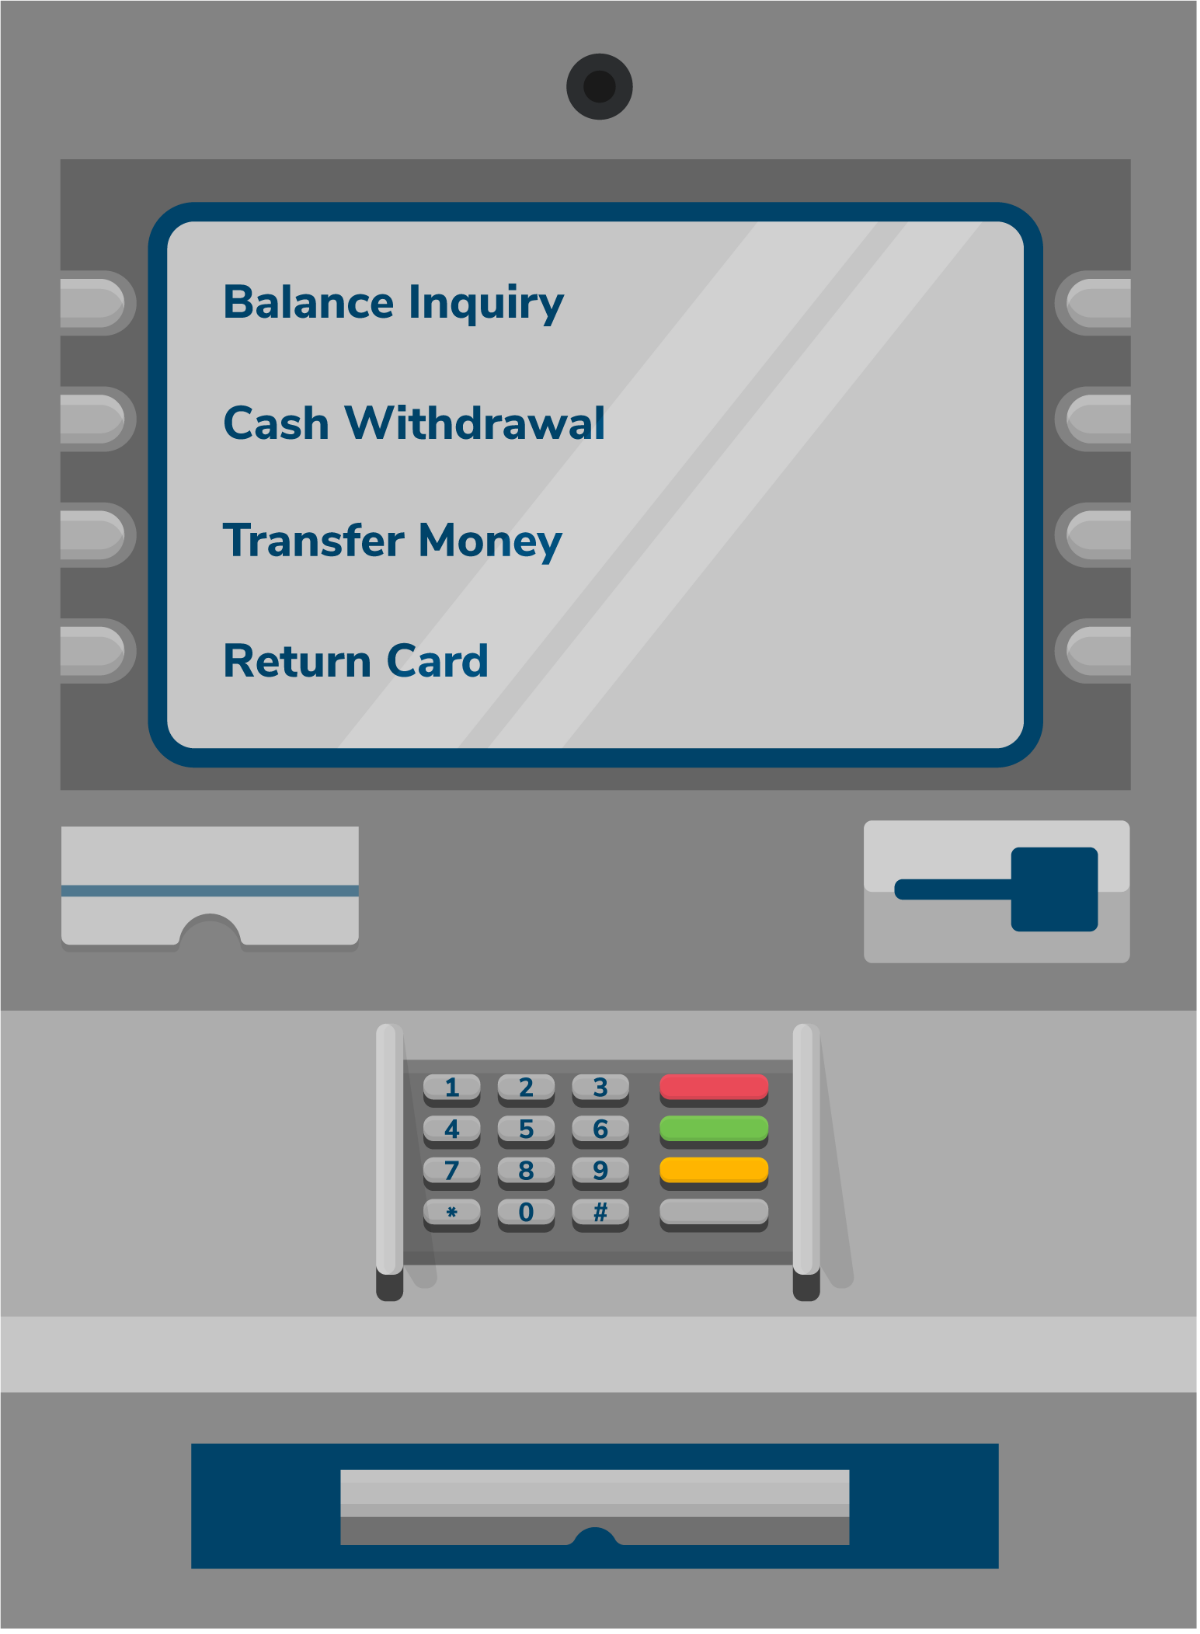
\includegraphics[width=\textwidth]{Images/chapter_16/section_5101998182760448/4912290735587328.png}
 \caption{The options above appear on the ATM upon successful PIN authentication}
 \end{subfigure}
 \hfill
 \begin{subfigure}[b]{0.48\textwidth}
 \centering
 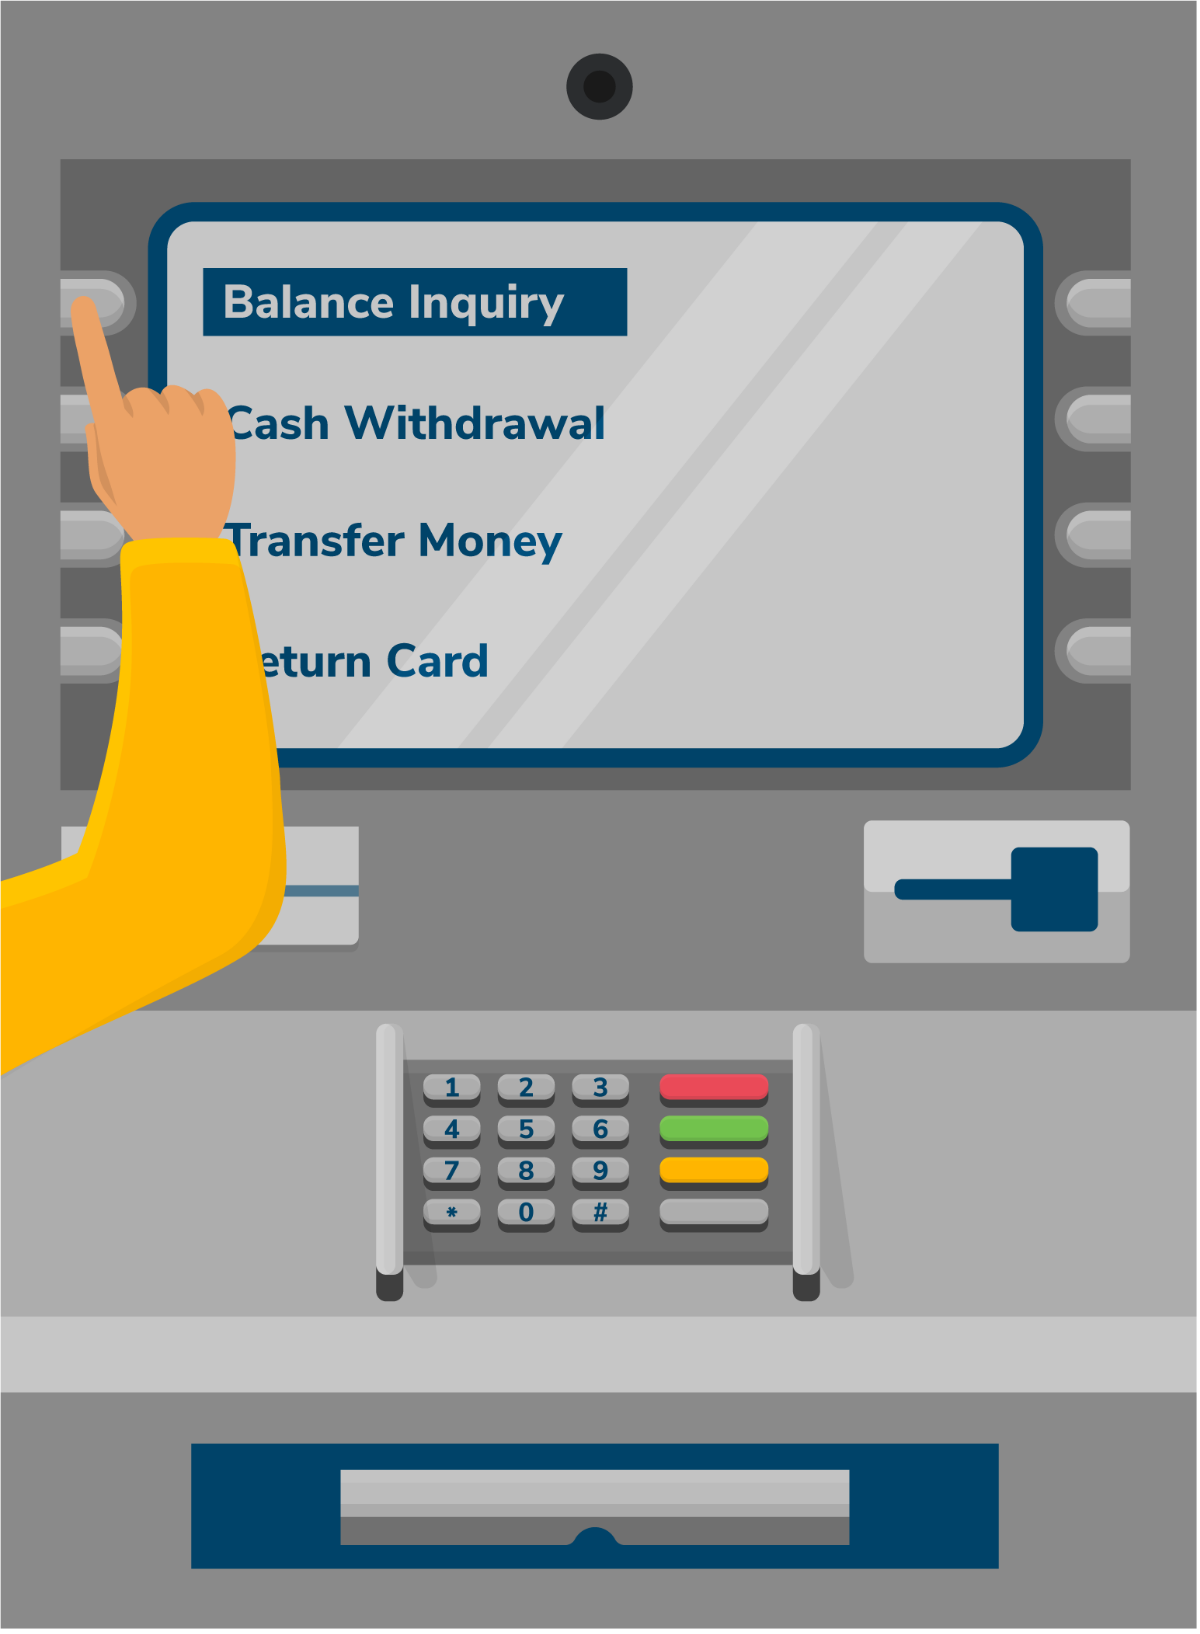
\includegraphics[width=\textwidth]{Images/chapter_16/section_5101998182760448/5076701265788928.png}
 \caption{The user selects the “Balance Inquiry” option}
 \end{subfigure}
\end{figure}

\begin{figure}[htbp]
 \centering
 \begin{subfigure}[b]{0.48\textwidth}
 \centering
 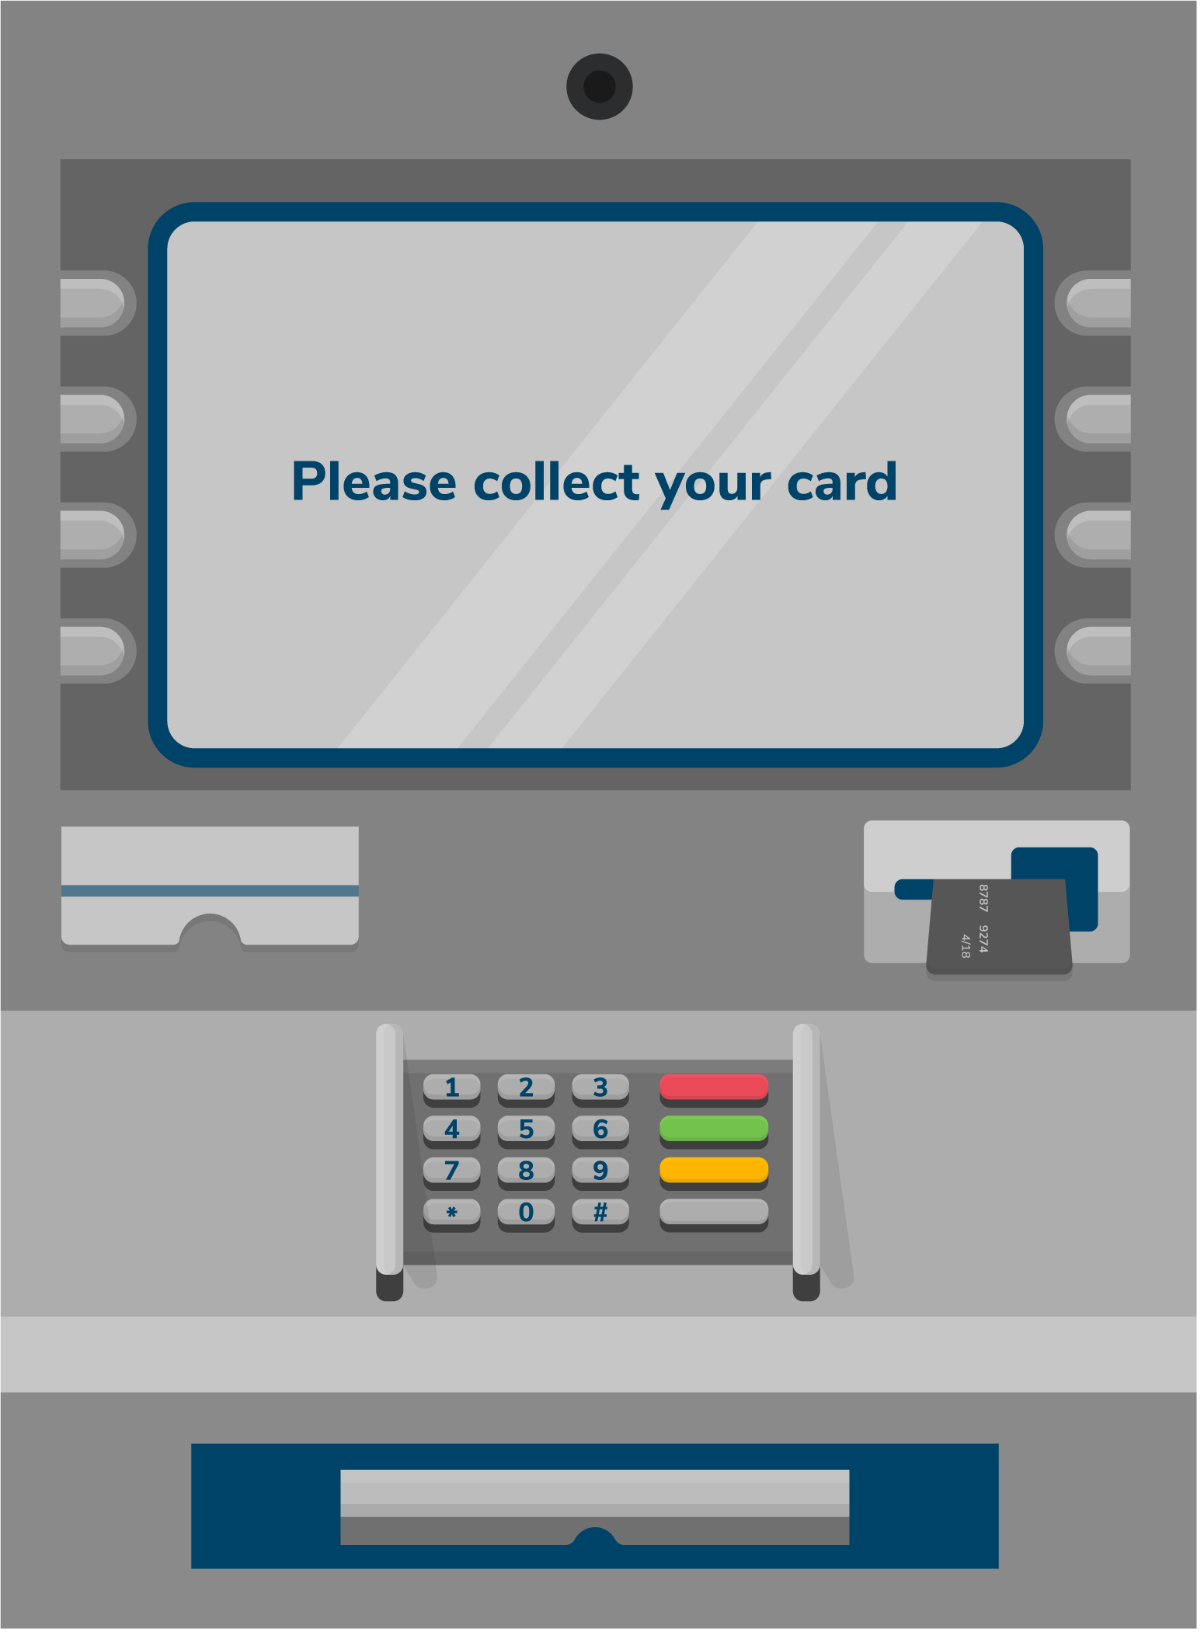
\includegraphics[width=\textwidth]{Images/chapter_16/section_5101998182760448/5035841895530496.png}
 \caption{The ATM asks the user to collect the card}
 \end{subfigure}
 \hfill
 \begin{subfigure}[b]{0.48\textwidth}
 \centering
 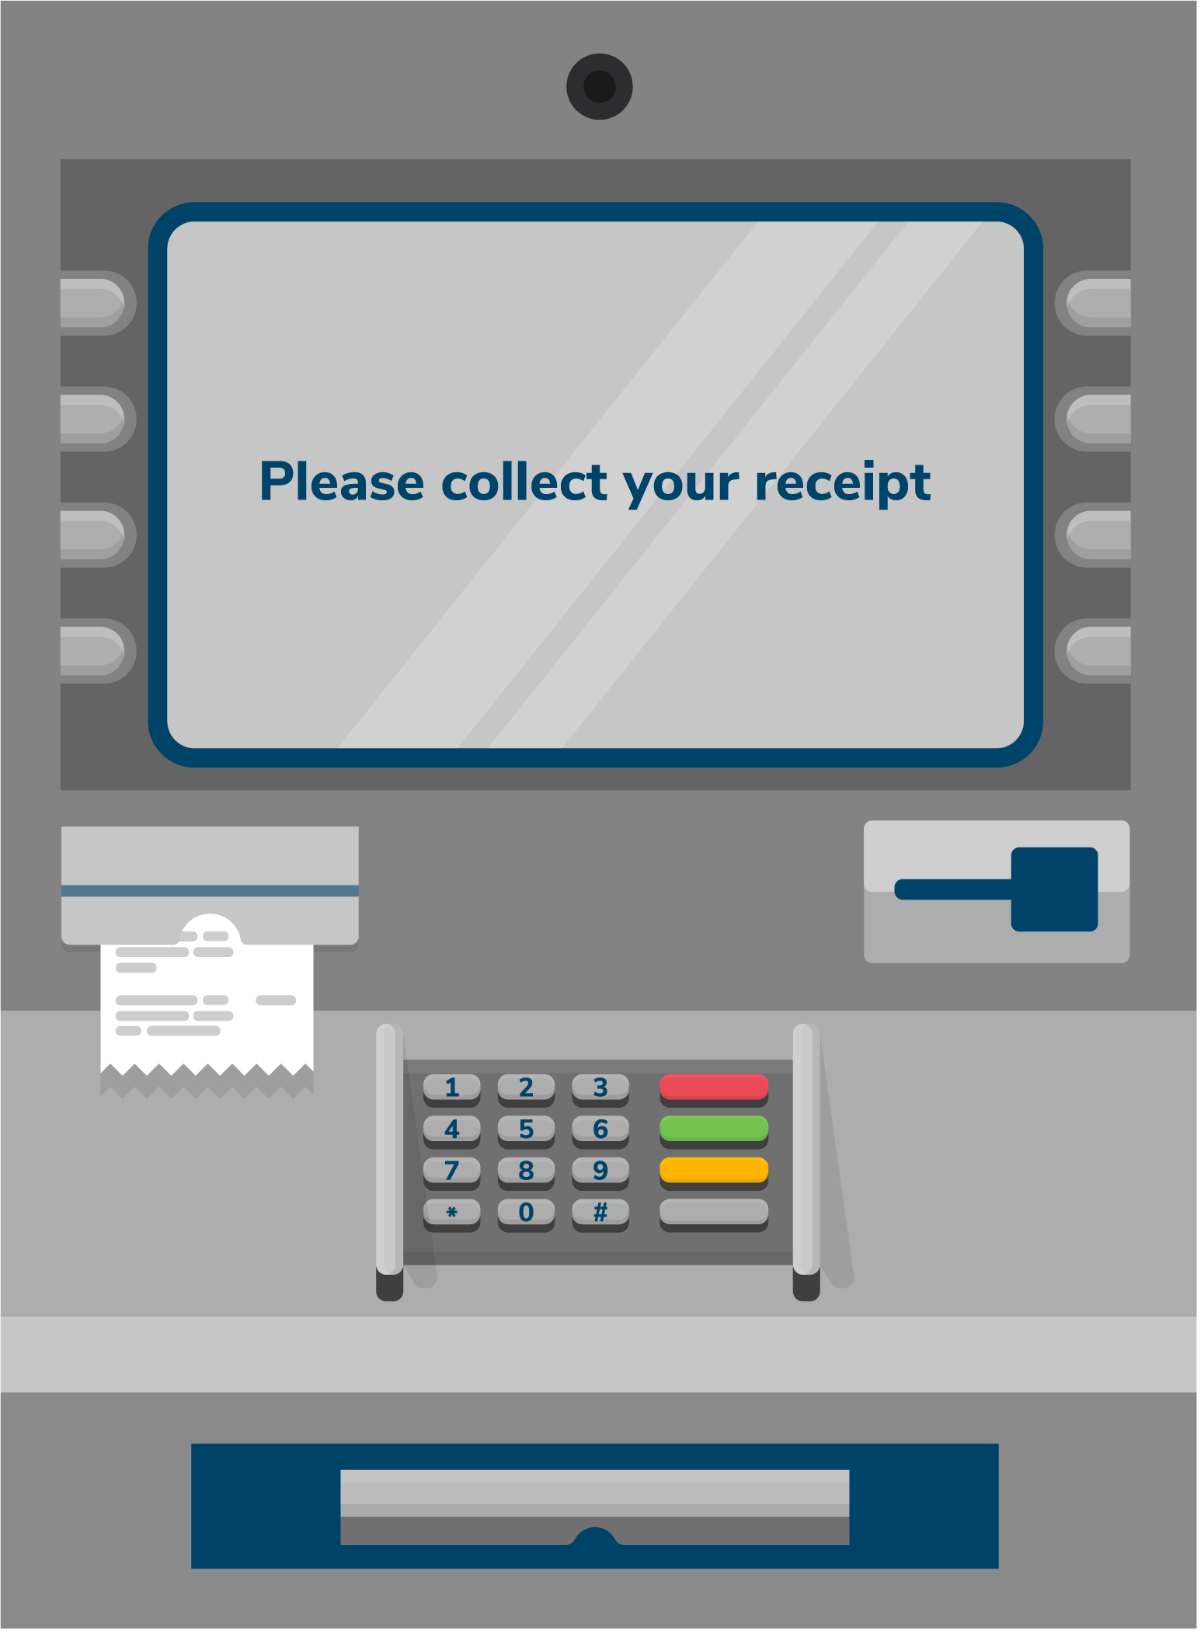
\includegraphics[width=\textwidth]{Images/chapter_16/section_5101998182760448/4666139851620352.png}
 \caption{The ATM asks the user to collect the balance receipt}
 \end{subfigure}
\end{figure}

\begin{figure}[htbp]
 \centering
 \begin{subfigure}[b]{0.48\textwidth}
 \centering
 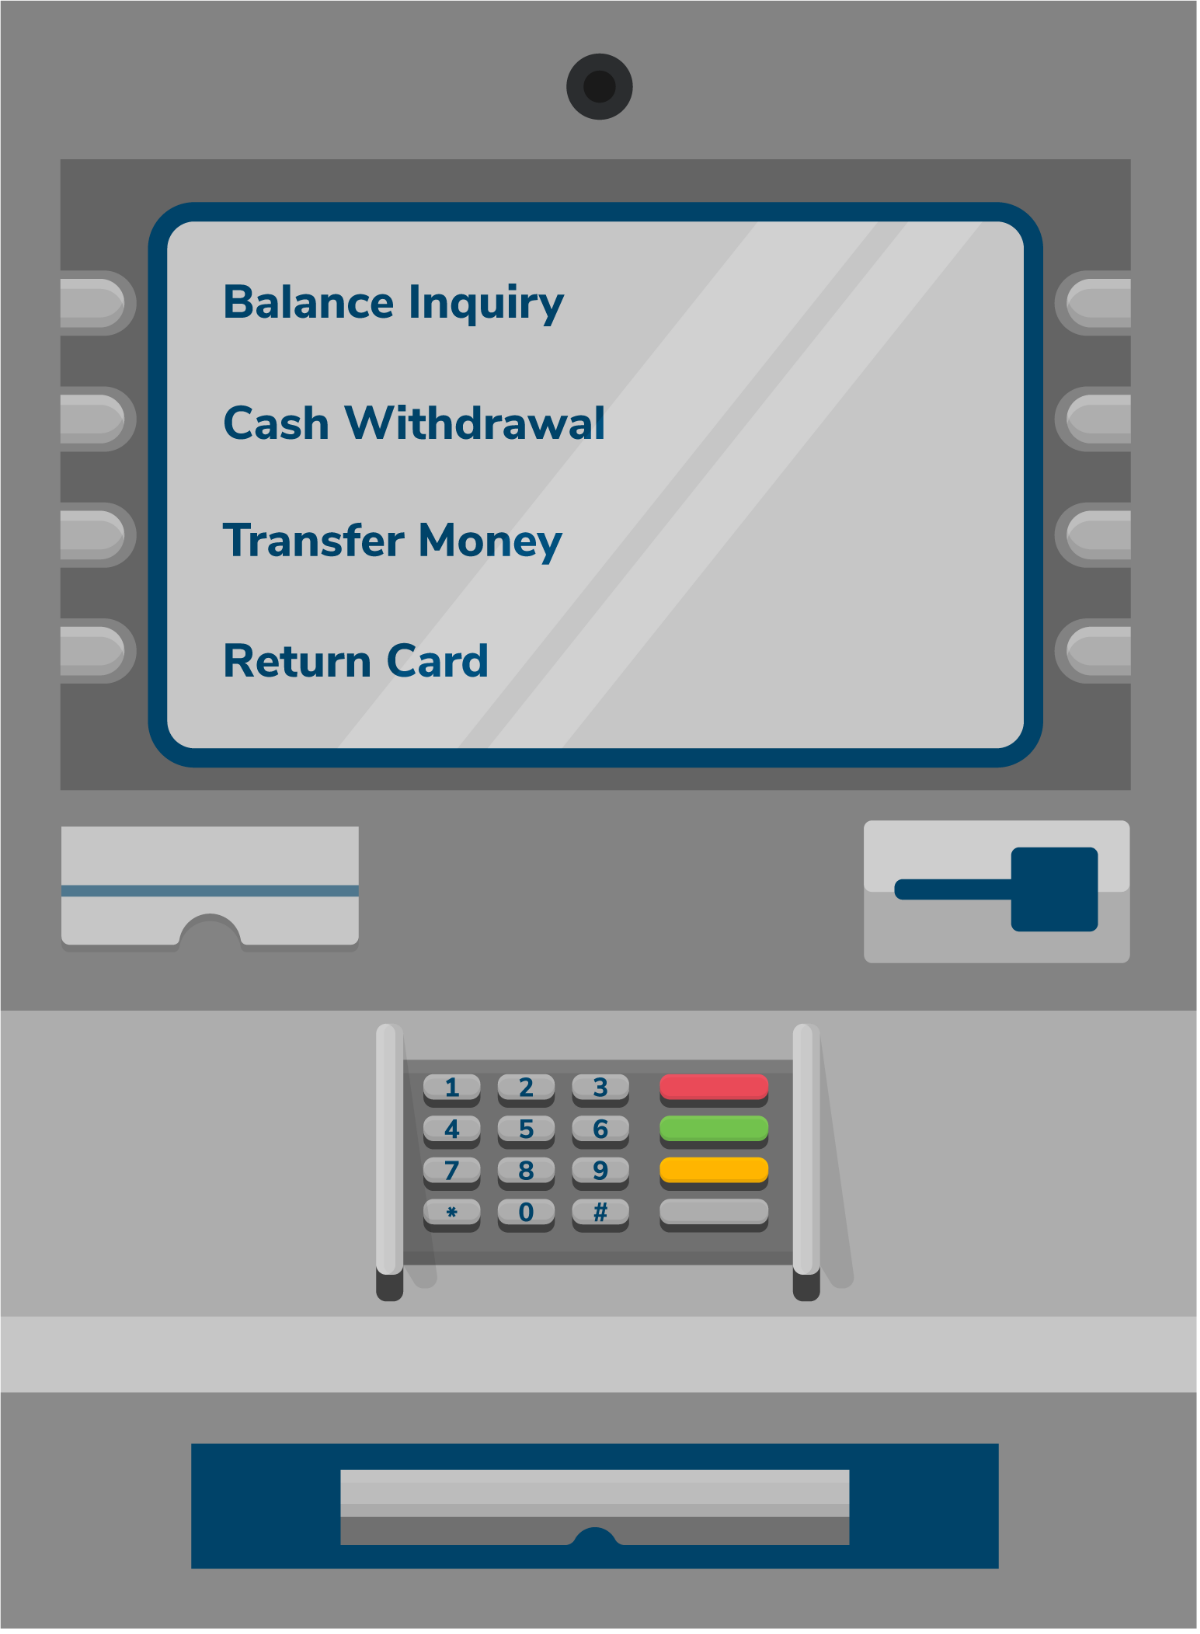
\includegraphics[width=\textwidth]{Images/chapter_16/section_5101998182760448/6209373677551616.png}
 \caption{The options above appear on the ATM upon successful PIN authentication}
 \end{subfigure}
 \hfill
 \begin{subfigure}[b]{0.48\textwidth}
 \centering
 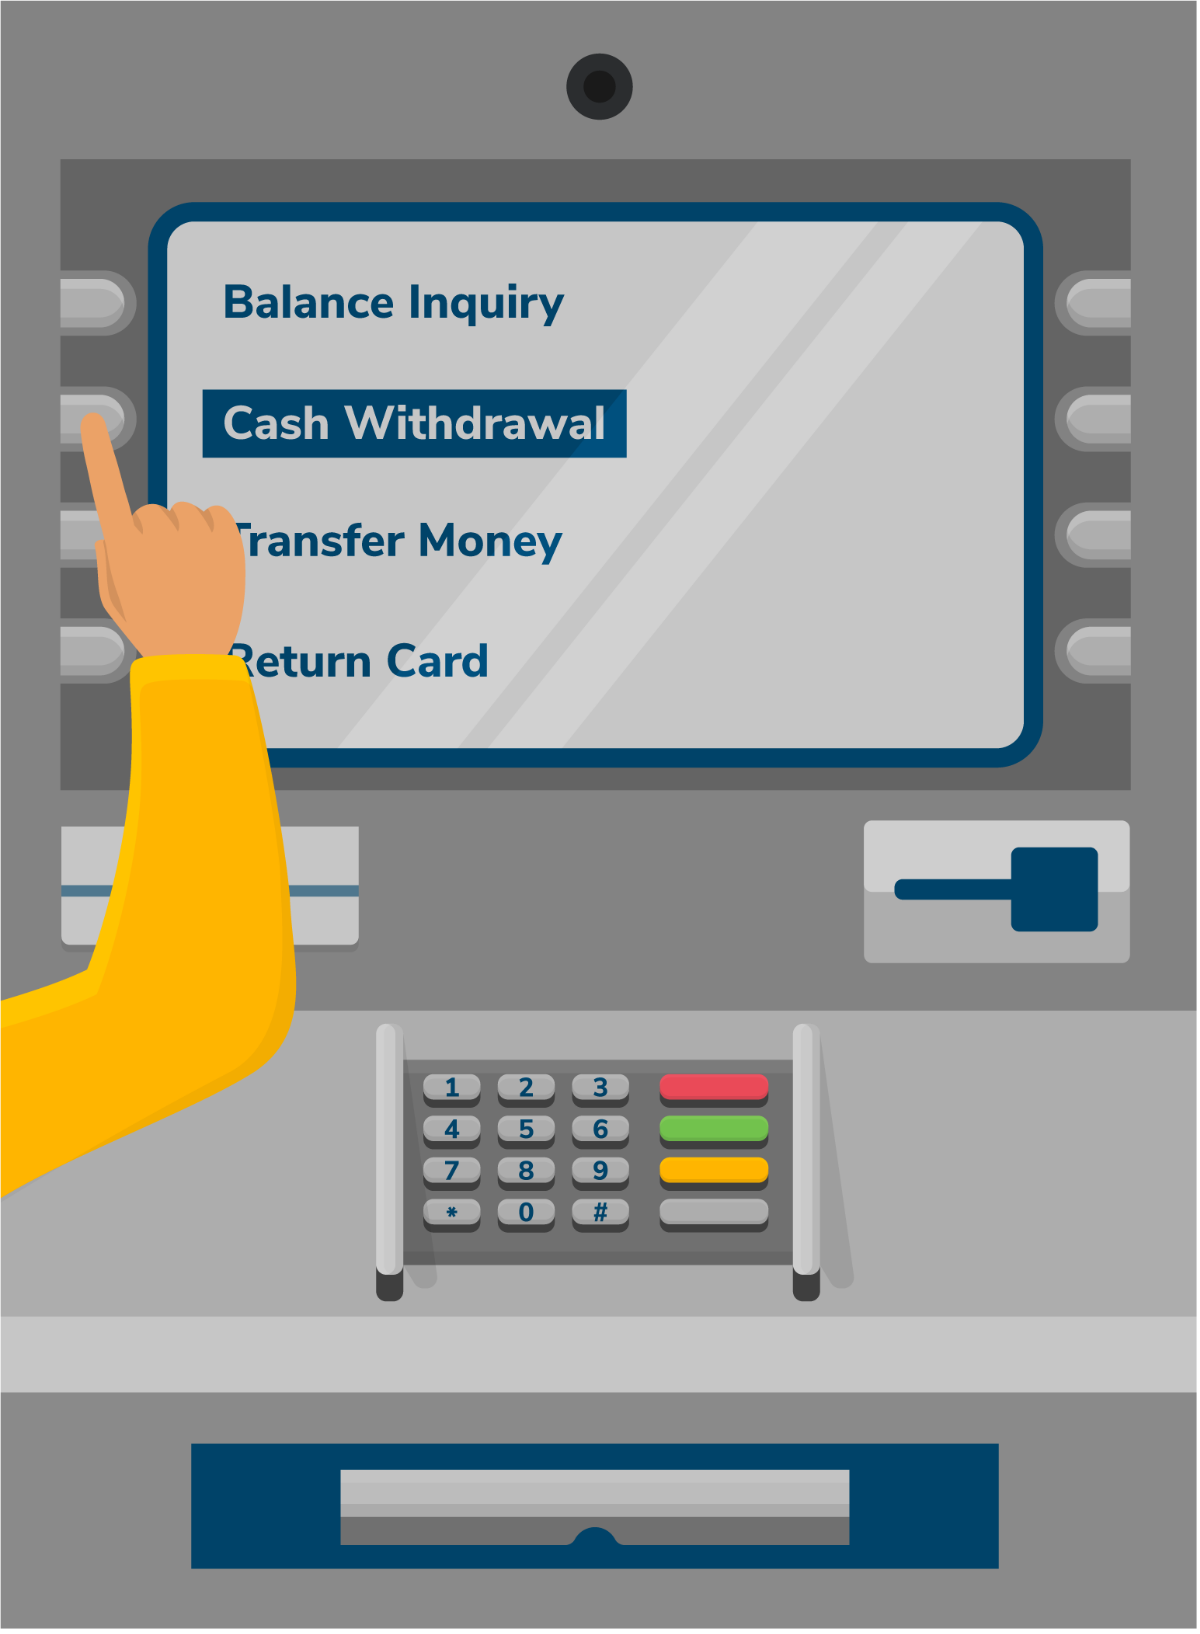
\includegraphics[width=\textwidth]{Images/chapter_16/section_5101998182760448/5140741774114816.png}
 \caption{The user selects the “Cash Withdrawal” option}
 \end{subfigure}
\end{figure}

\begin{figure}[htbp]
 \centering
 \begin{subfigure}[b]{0.48\textwidth}
 \centering
 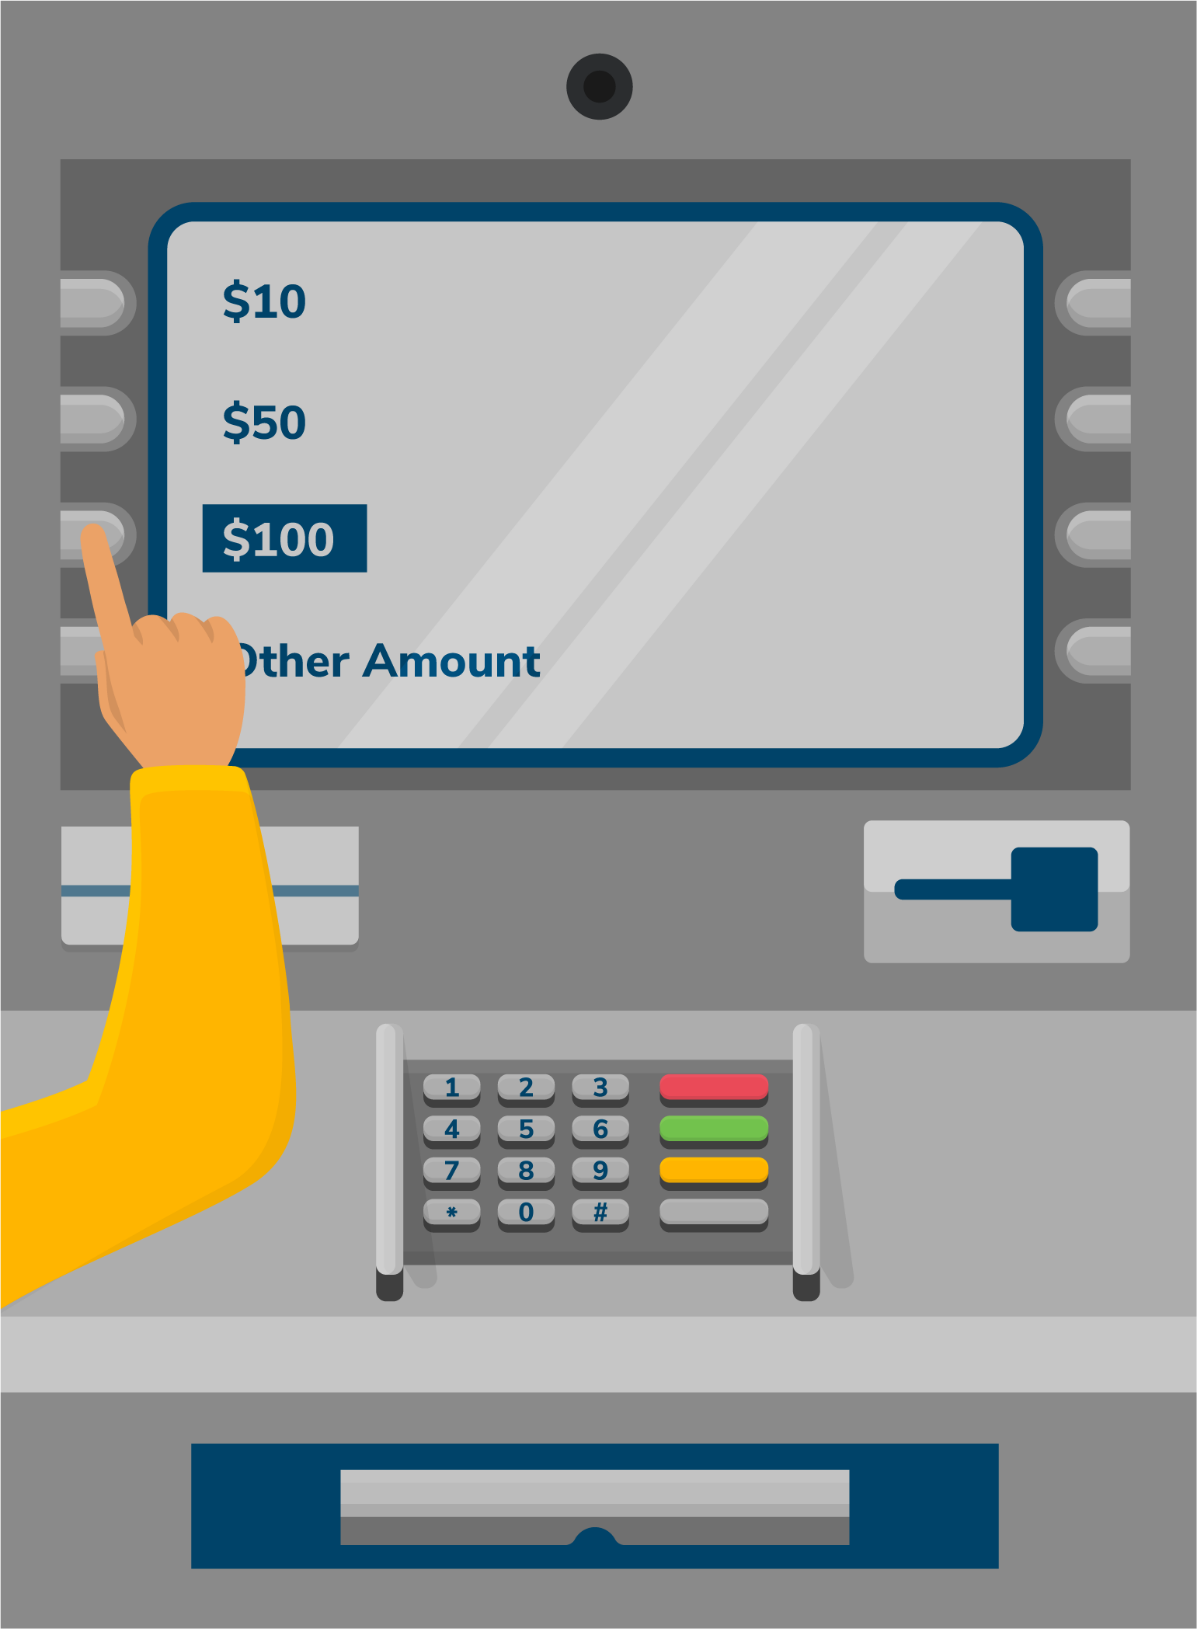
\includegraphics[width=\textwidth]{Images/chapter_16/section_5101998182760448/6124758258417664.png}
 \caption{The user selects the “\$100” option}
 \end{subfigure}
 \hfill
 \begin{subfigure}[b]{0.48\textwidth}
 \centering
 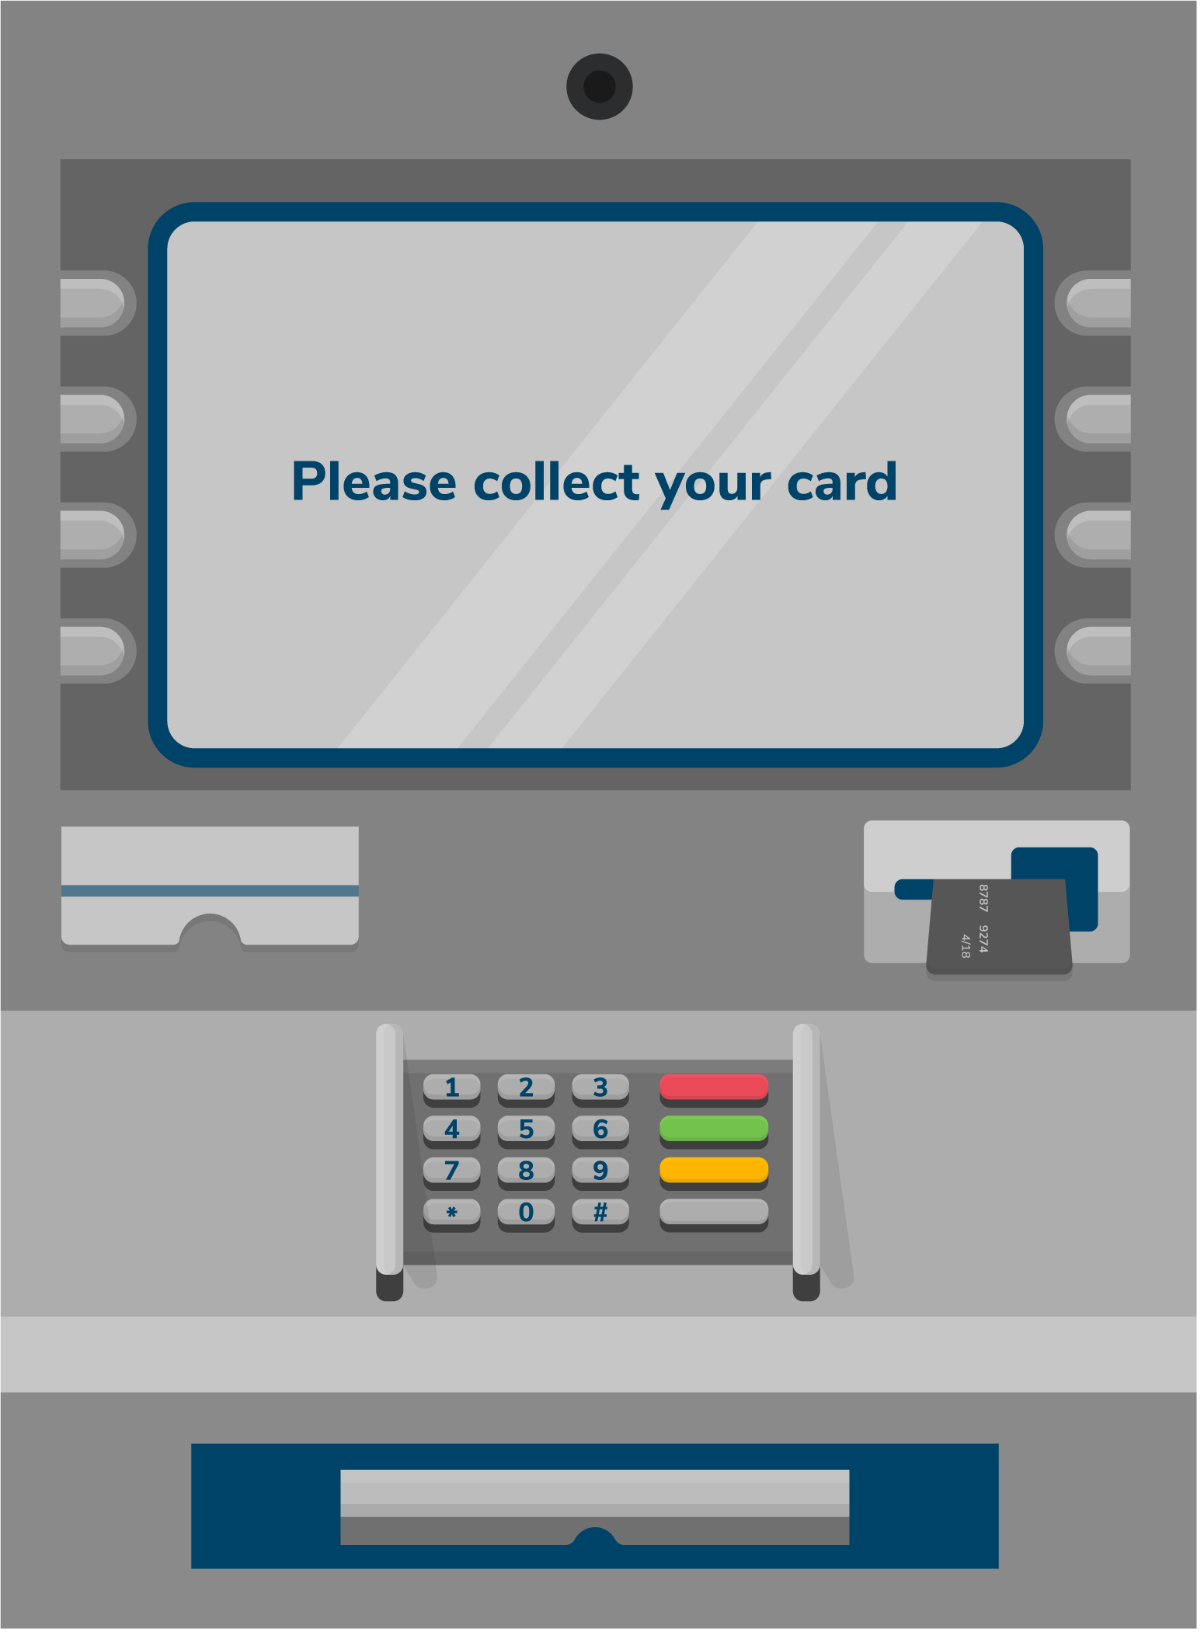
\includegraphics[width=\textwidth]{Images/chapter_16/section_5101998182760448/6287101562978304.png}
 \caption{The ATM asks the user to collect the card}
 \end{subfigure}
\end{figure}

\begin{figure}[htbp]
 \centering
 \begin{subfigure}[b]{0.48\textwidth}
 \centering
 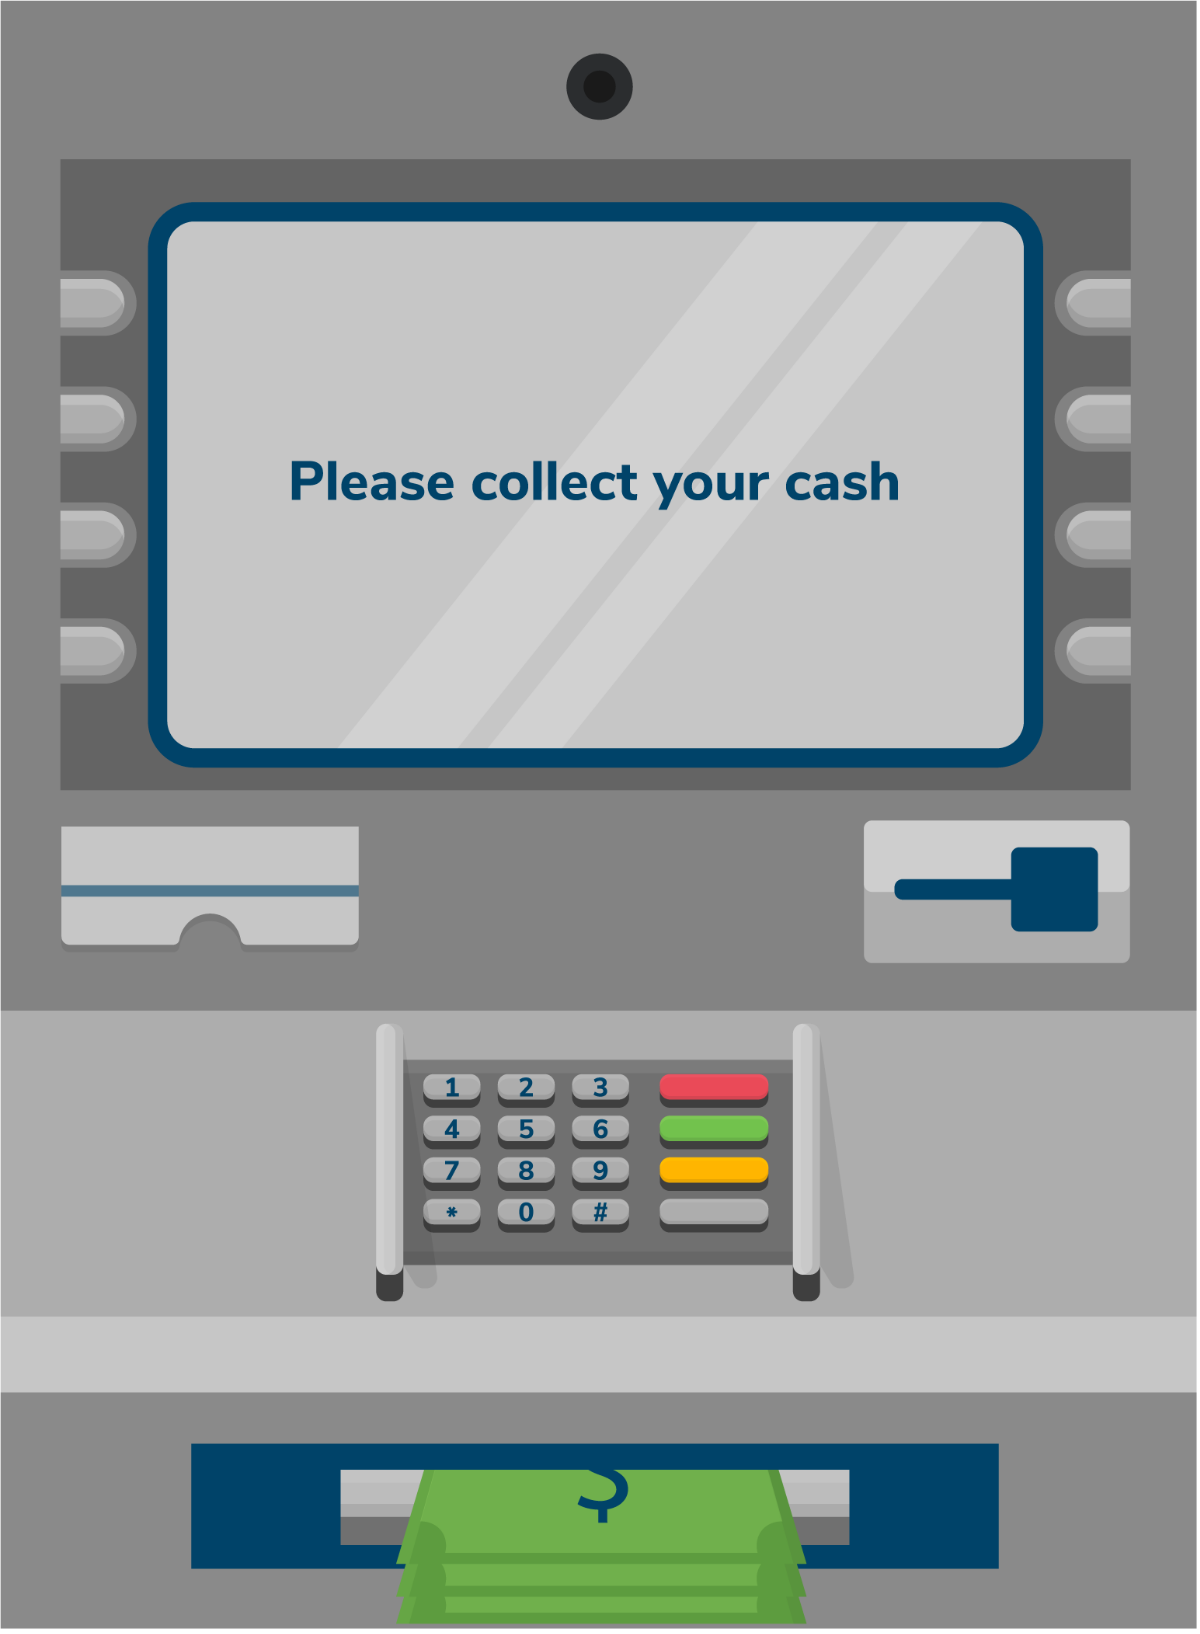
\includegraphics[width=\textwidth]{Images/chapter_16/section_5101998182760448/5167324970876928.png}
 \caption{The ATM asks the user to collect the cash according to the amount specified}
 \end{subfigure}
 \hfill
 \begin{subfigure}[b]{0.48\textwidth}
 \centering
 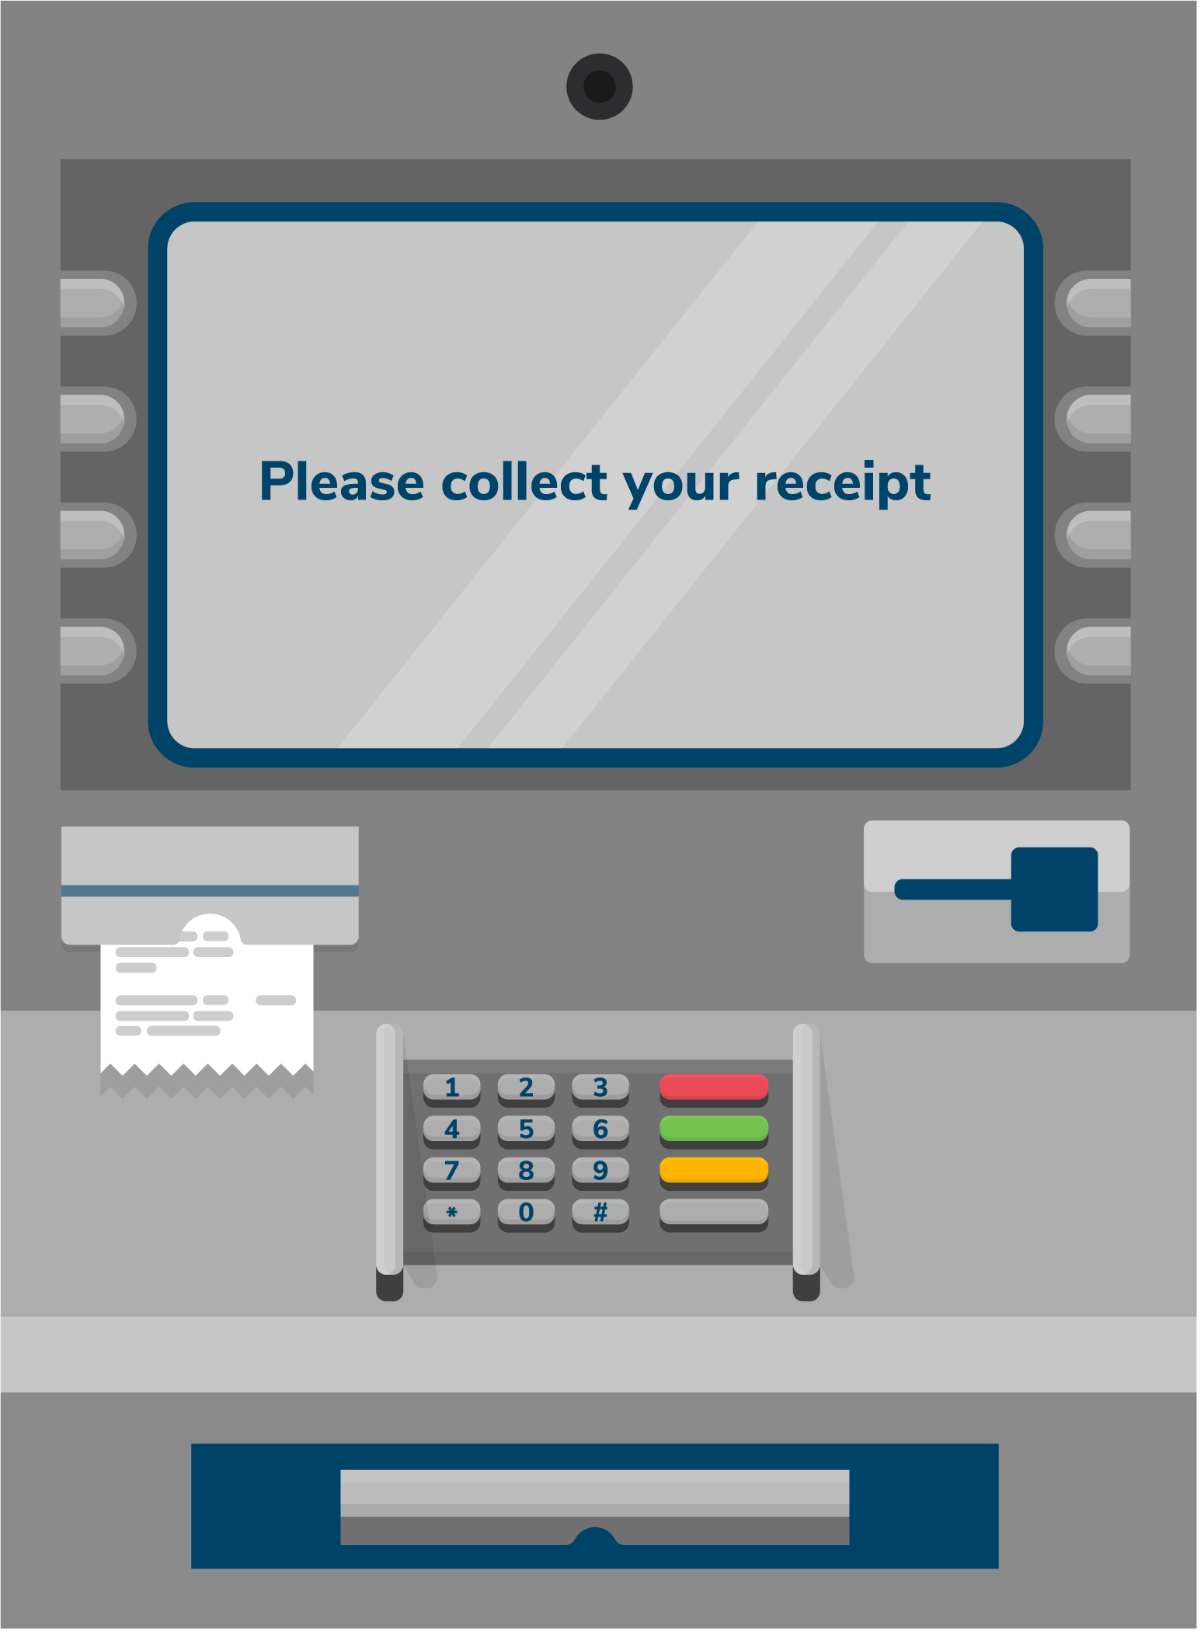
\includegraphics[width=\textwidth]{Images/chapter_16/section_5101998182760448/6180849323343872.png}
 \caption{The ATM asks the user to collect the receipt}
 \end{subfigure}
\end{figure}

\begin{figure}[htbp]
 \centering
 \begin{subfigure}[b]{0.48\textwidth}
 \centering
 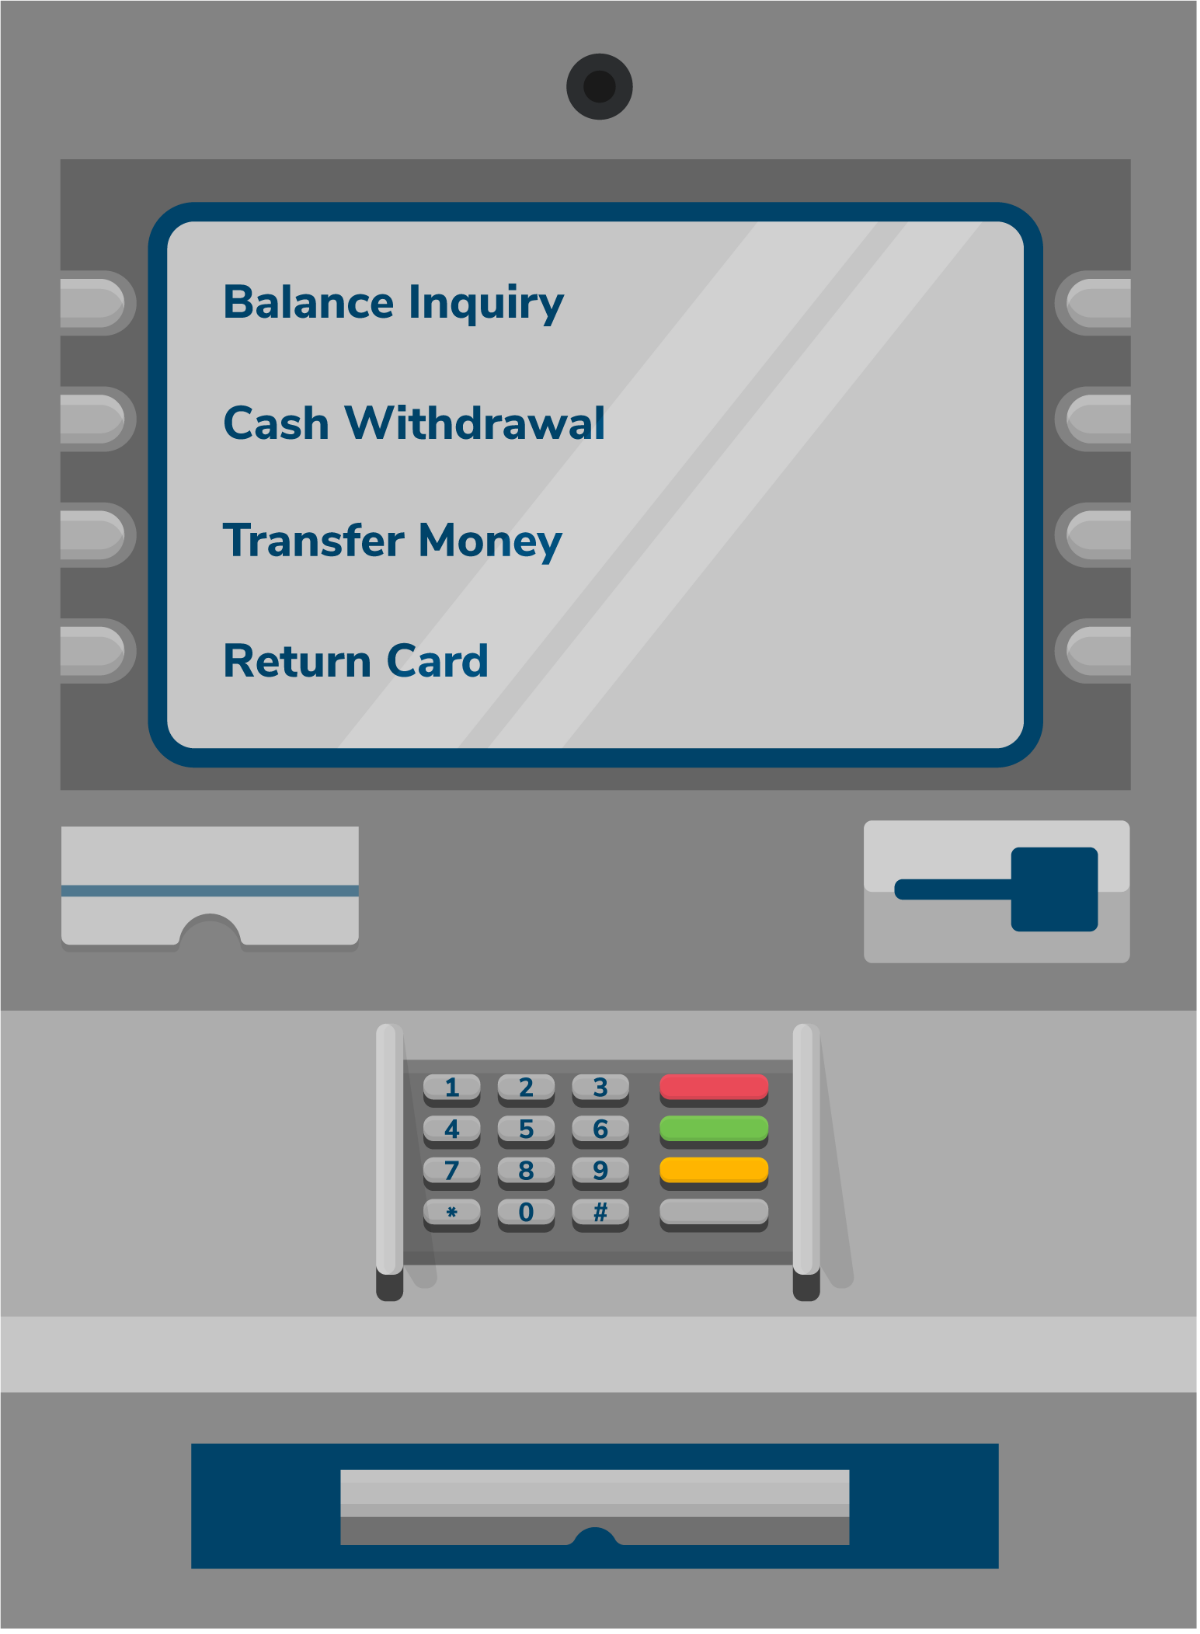
\includegraphics[width=\textwidth]{Images/chapter_16/section_5101998182760448/4663816261730304.png}
 \caption{The options that appear on the ATM upon successful PIN authentication}
 \end{subfigure}
 \hfill
 \begin{subfigure}[b]{0.48\textwidth}
 \centering
 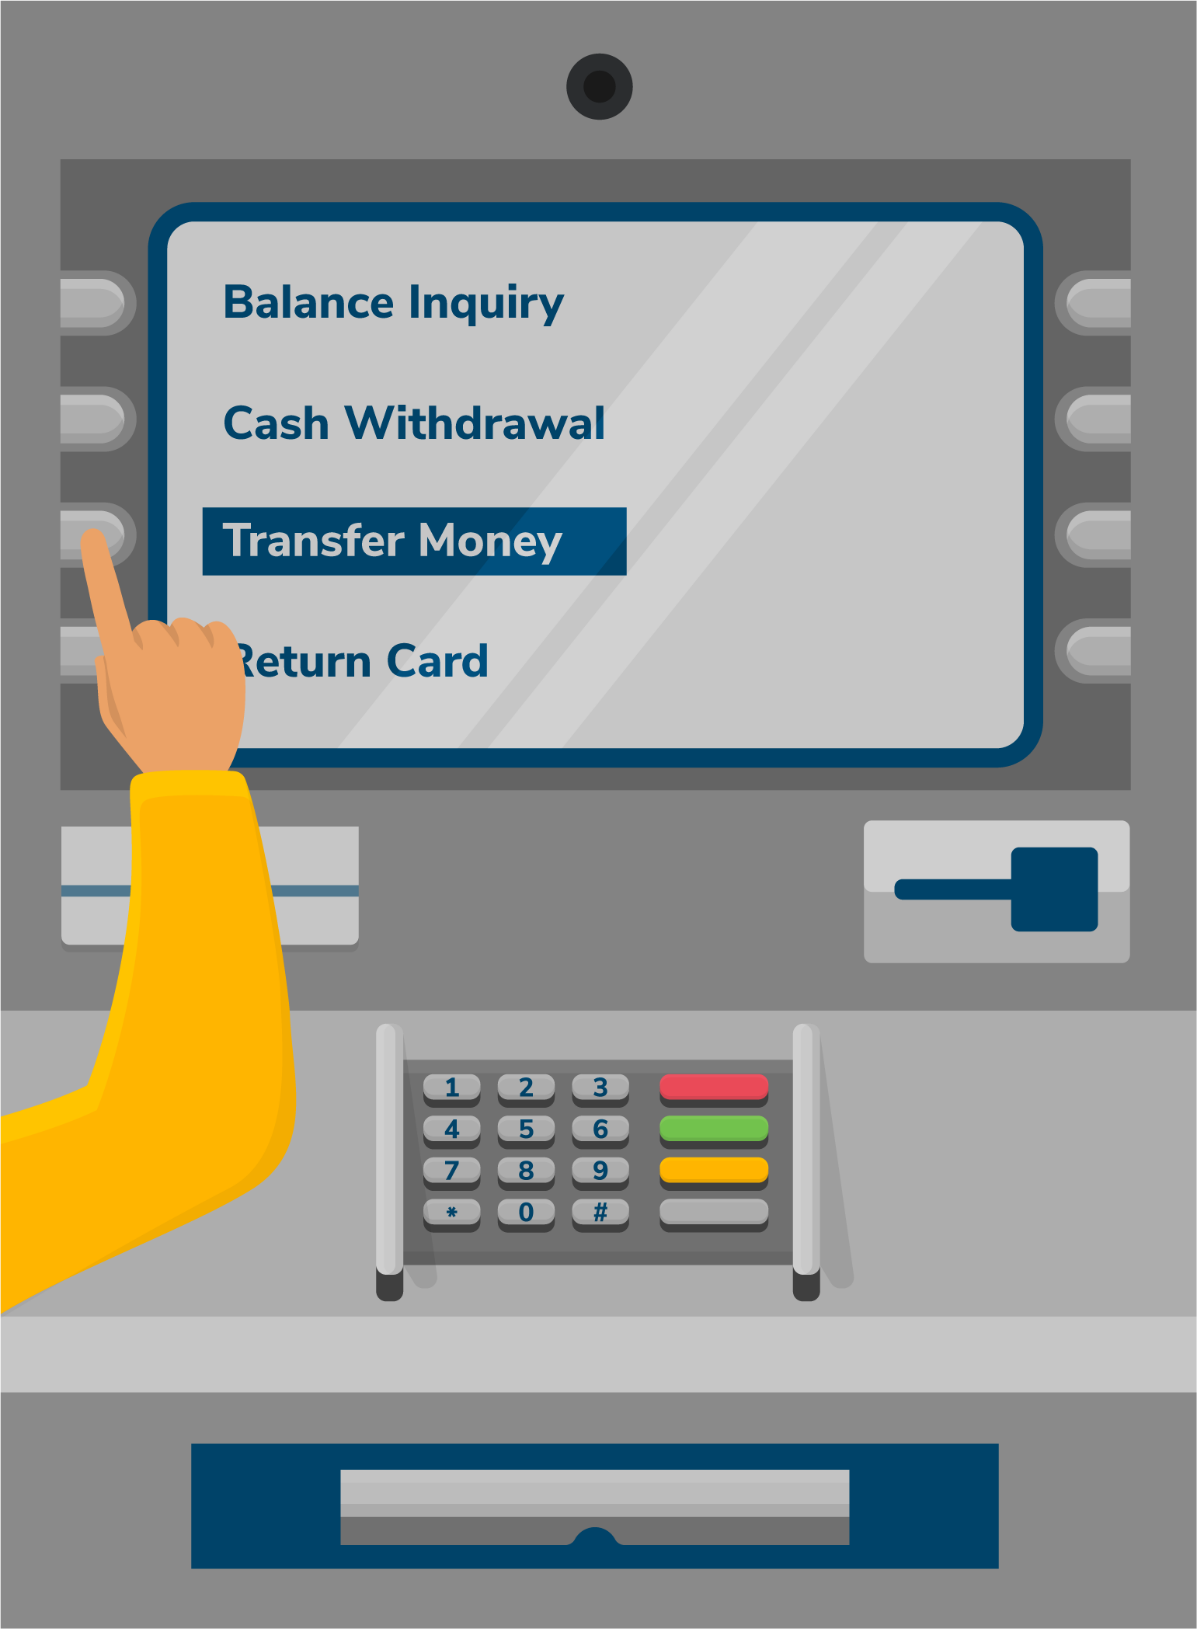
\includegraphics[width=\textwidth]{Images/chapter_16/section_5101998182760448/5645744867639296.png}
 \caption{The user selects the "Transfer Money" option}
 \end{subfigure}
\end{figure}

\begin{figure}[htbp]
 \centering
 \begin{subfigure}[b]{0.48\textwidth}
 \centering
 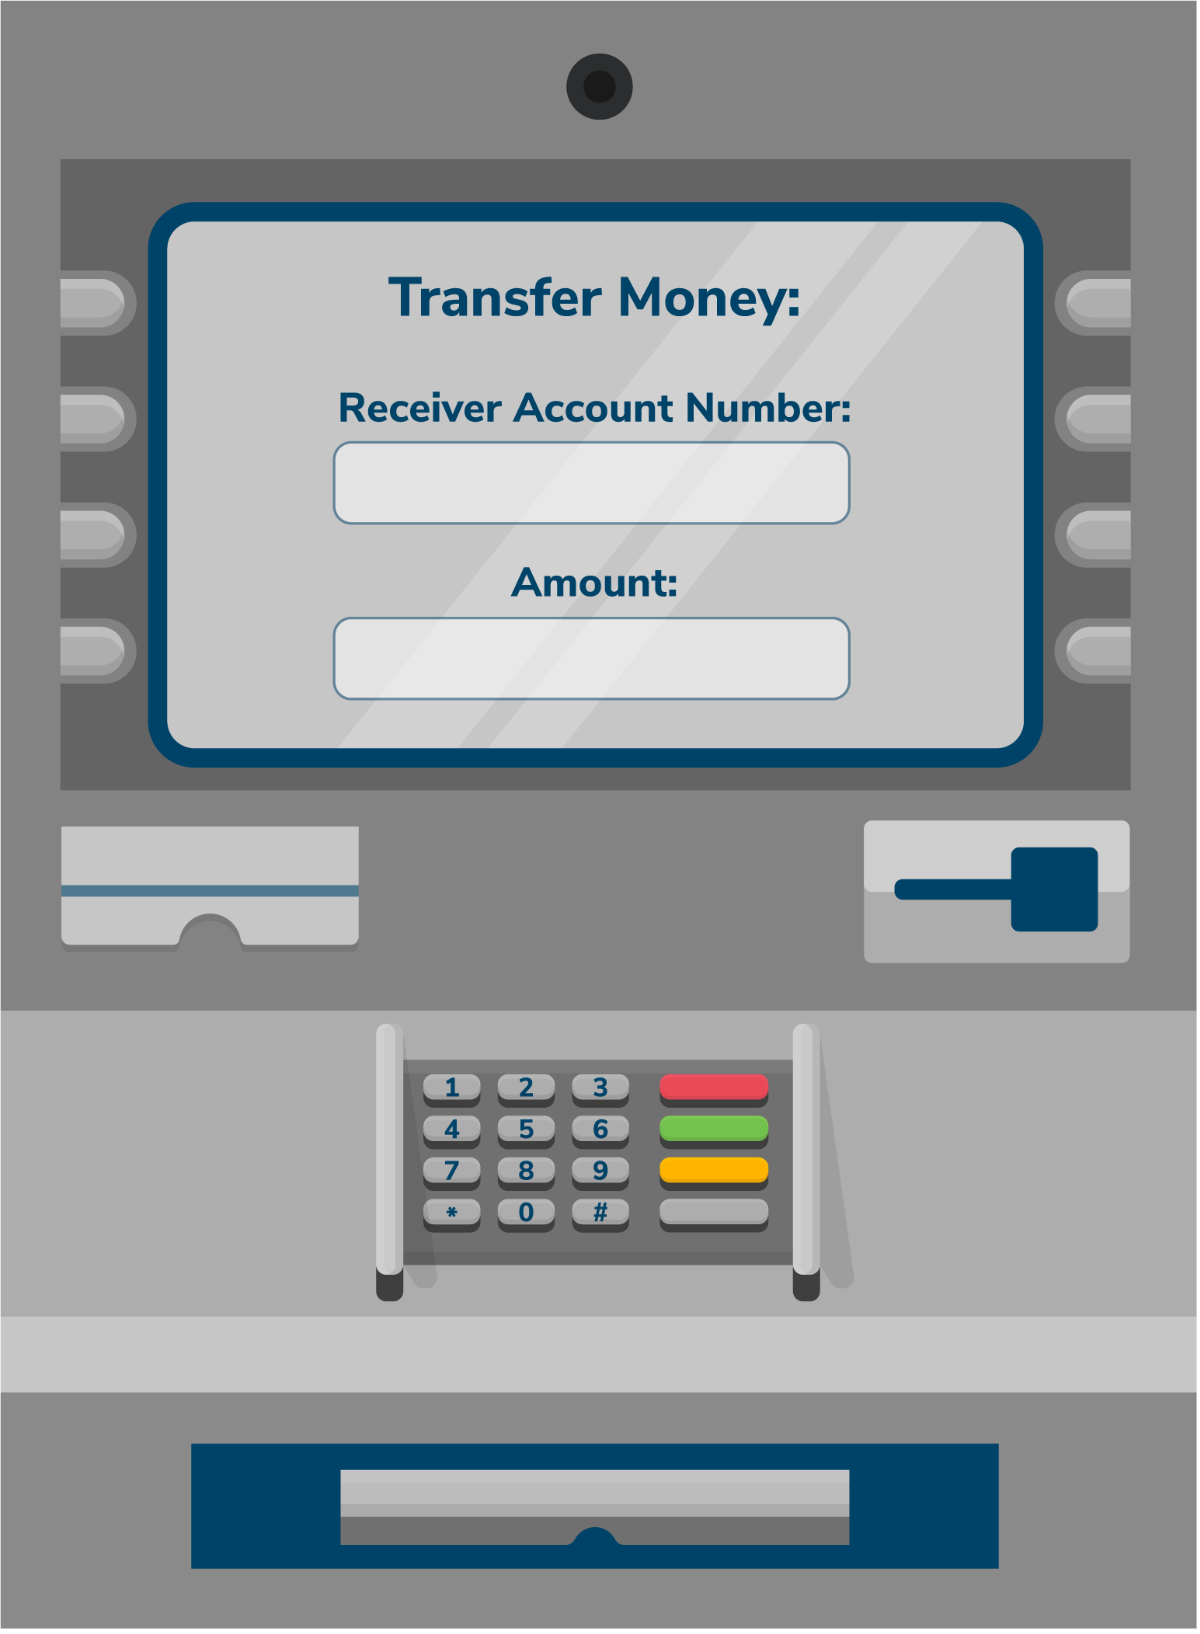
\includegraphics[width=\textwidth]{Images/chapter_16/section_5101998182760448/5740743420542976.png}
 \caption{The ATM prompts the user to enter the receiver account number and the amount to be sent}
 \end{subfigure}
 \hfill
 \begin{subfigure}[b]{0.48\textwidth}
 \centering
 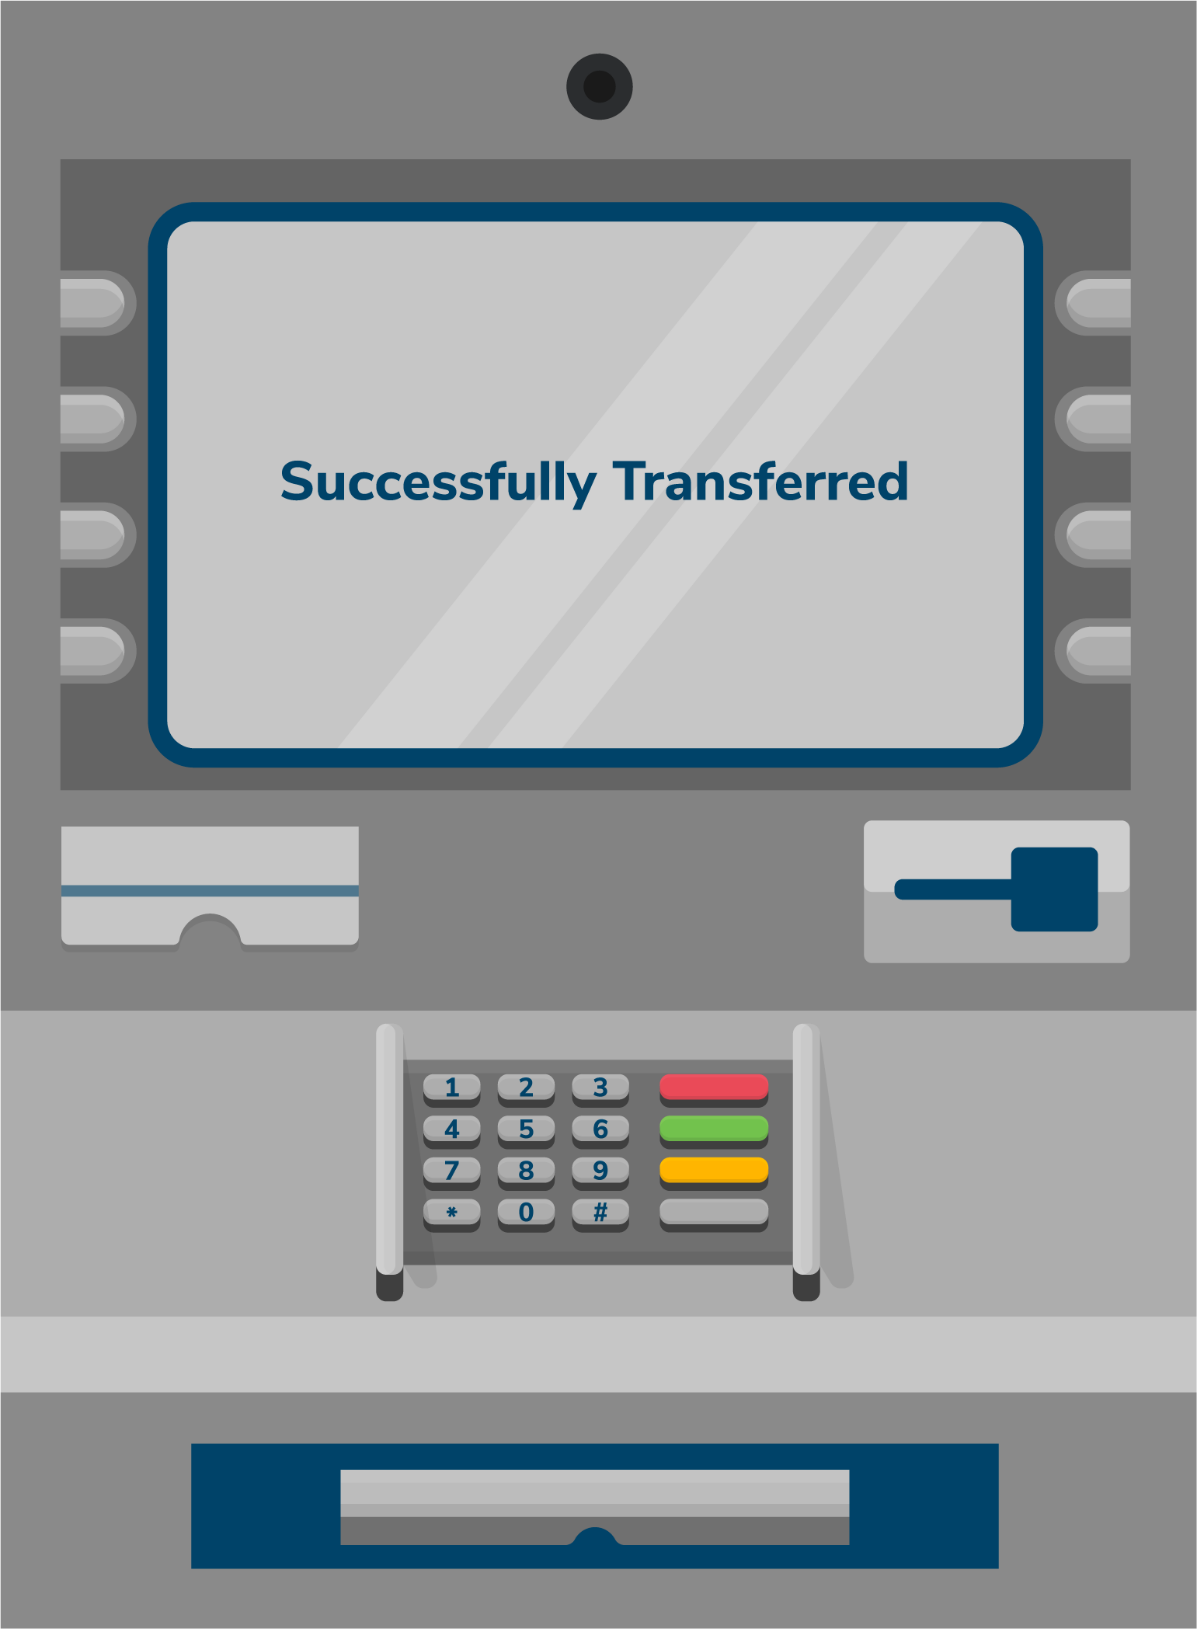
\includegraphics[width=\textwidth]{Images/chapter_16/section_5101998182760448/5099976846999552.png}
 \caption{The ATM notifies the user that the transaction was successful}
 \end{subfigure}
\end{figure}

\begin{figure}[htbp]
 \centering
 \begin{subfigure}[b]{0.48\textwidth}
 \centering
 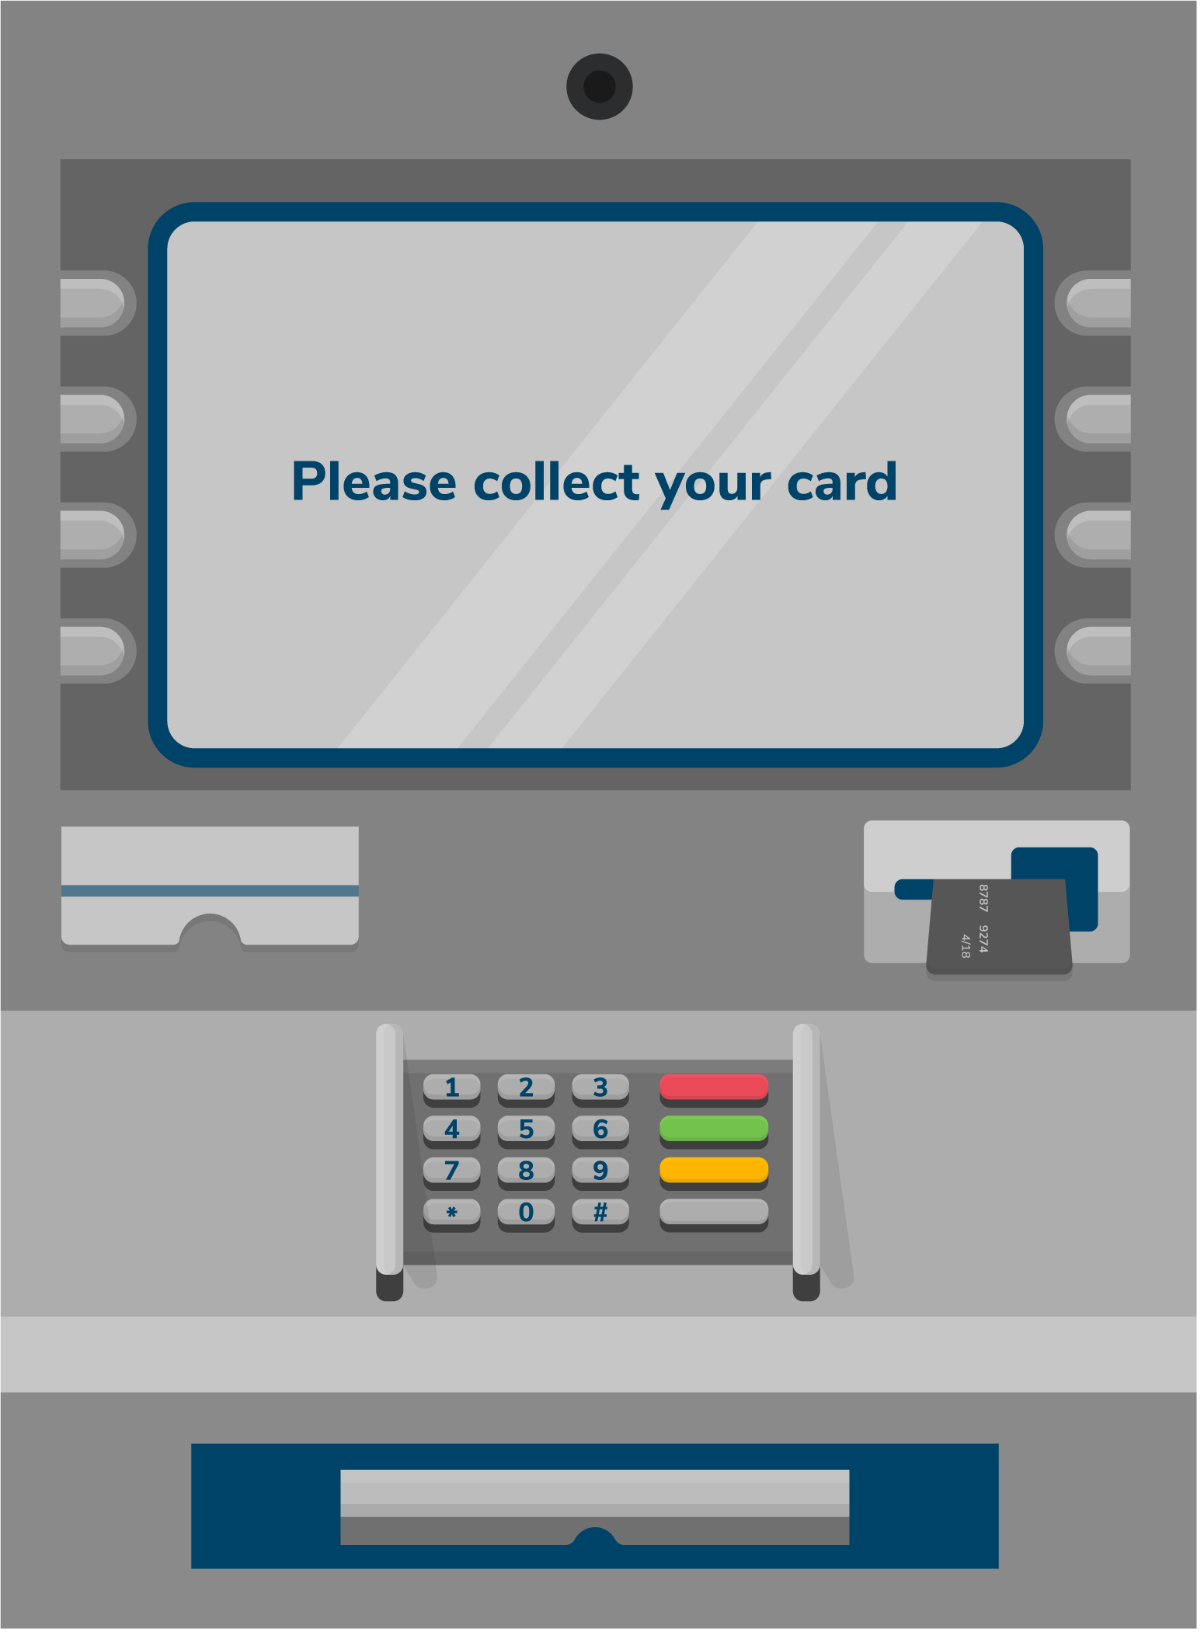
\includegraphics[width=\textwidth]{Images/chapter_16/section_5101998182760448/6287101562978304.png}
 \caption{The ATM asks the user to collect the card}
 \end{subfigure}
 \hfill
 \begin{subfigure}[b]{0.48\textwidth}
 \centering
 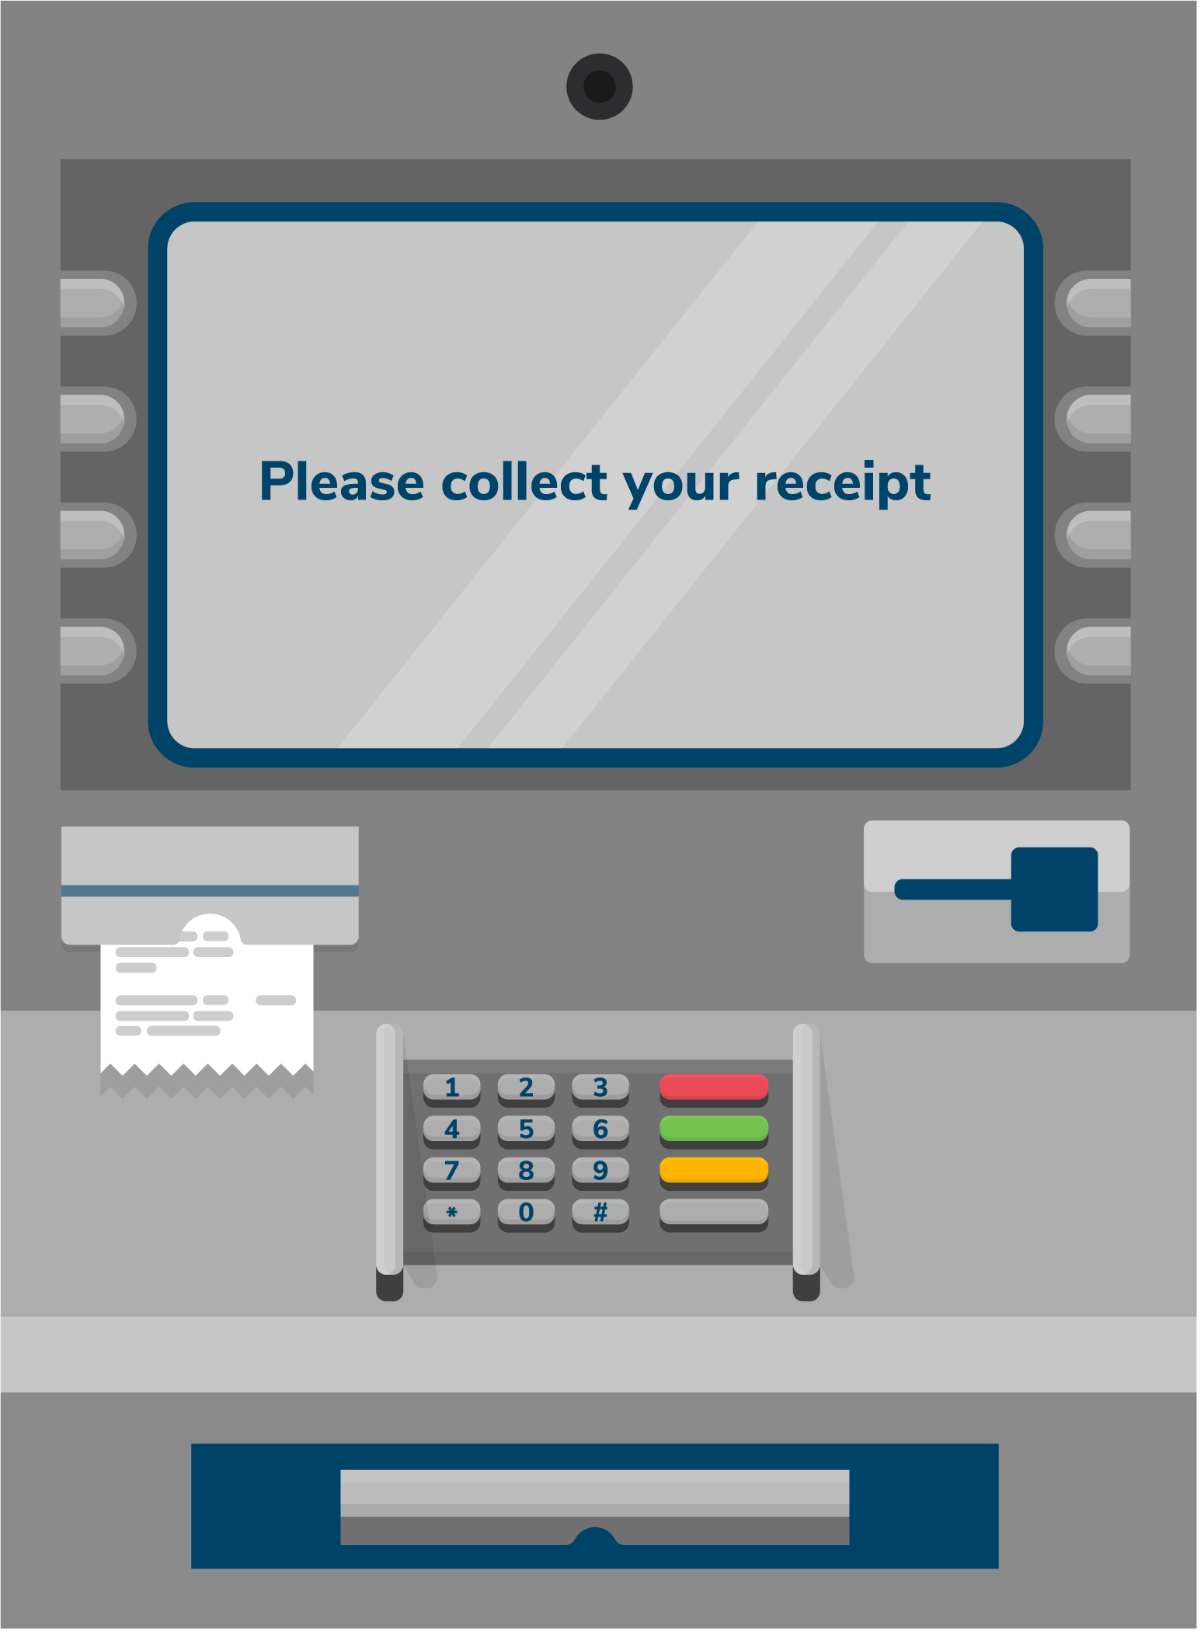
\includegraphics[width=\textwidth]{Images/chapter_16/section_5101998182760448/6180849323343872.png}
 \caption{The ATM asks the user to collect the receipt}
 \end{subfigure}
\end{figure}

\subsection{Expectations from the interviewee}\label{A0ToqGogbV0I93ewZZ4Yg}
\\
During the interview, you are expected to discuss key aspects of the ATM system's design, clarifying requirements, handling edge cases, and reasoning about hardware-software interactions. Typical areas to cover include:

\subsubsection{ATM components}\label{HXFQHgPGBVL3VJAhkRdkA}
\\
To better understand an ATM system, you may ask the interviewer the following questions:

\begin{enumerate}
\item
\protect\phantomsection\label{GoM1mgtvRy9MhdZCMOWpO}
What are the components of an ATM?
\item
\protect\phantomsection\label{P02IAljGvMyLm_DIWPvu3}
Is the ATM necessarily placed inside a room?
\item
\protect\phantomsection\label{R8yFDj_i51HWyLwvN0ZX0}
Does an ATM have a fingerprint scanner?
\end{enumerate}

\subsubsection{ATM features}\label{mTmk9GwFZQC4f3vC5NhBP}
\\
Different ATMs may vary in terms of features, which is why it is important to clear the following questions from the interviewer:

\begin{enumerate}
\item
\protect\phantomsection\label{E34MgfwnYhQhOMy-fsqmU}
What is the withdrawal limit of an ATM?
\item
\protect\phantomsection\label{cBDgPPQfFz18lom24D-XQ}
Can we check our account balance using an ATM?
\item
\protect\phantomsection\label{T4vEX1oAp0FmOHCEDyVOK}
Can we set a PIN using an ATM?
\end{enumerate}

\subsubsection{ATM processing}\label{fgILgnm2bTHPC4sdWONjZ}
\\
The interviewer would expect you to ask a question about processing ATM transactions. Therefore, you may ask the following questions:

\begin{enumerate}
\item
What happens when the amount the user enters for withdrawal exceeds the user's account balance?
\item
What happens when the amount the user enters for withdrawal exceeds the ATM's cash limit?
\item
What happens when the amount the user enters exceeds the total cash in the ATM?
\item
Can the ATM be used for online transactions?
\end{enumerate}

\subsection{Design approach}\label{D06nks8FfR2O_xpSVW1A-}
\\
We will design this ATM system using a \emph{bottom-up approach}, following these steps:

\begin{itemize}
\item
\protect\phantomsection\label{_KOjJNDy660ZuE758FoJU}
First, we'll identify and model the core hardware components such as \texttt{CardReader}, \texttt{Keypad}, \texttt{Screen}, \texttt{CashDispenser}, and \texttt{Printer}, defining their responsibilities and interactions.
\item
\protect\phantomsection\label{S4ORq9QdSR3fOI60iqNnB}
Next, we'll compose these components into larger entities representing the ATM's operational state, transaction workflows, and the overall machine.
\item
\protect\phantomsection\label{qkPa1nXbkB0ji4KowjrqB}
We'll model how the ATM interacts with users for authentication, processes various transactions, manages its cash inventory, and ensures secure and reliable operations.
\item
\protect\phantomsection\label{ZTwp7jGf1t3gl0BIQI2Fd}
This approach will allow us to address edge cases, hardware failures, and incorporate SOLID design principles for modularity and maintainability. We 'll use diagrams and code examples to illustrate the design at each step.
\end{itemize}

\subsection{Design pattern~}\label{Tl3CBEntZg8Htk50fc3i7}
\\
During an interview, discussing the design patterns under which the ATM system falls is always a good practice. Stating the design patterns gives the interviewer a positive impression and shows that the interviewee is well-versed in the advanced concepts of object-oriented design.
\\
Try to answer the following question. If you are not familiar with design patterns, don't worry! You can learn about them by asking, ``Define design patterns.''

\textbf{Question:}

Which design pattern(s) should be used to design an ATM system? Please elaborate on your choice(s).

Let's explore the requirements of the ATM system in the next lesson.

\subsection{}\label{O2Rf8oUfIWpiPVHb-pkAy}

% End of section content